\chapter{Results and Discussion}\label{ResultsDiscussion}

This chapter presents the results from the experiments described in the \ref{Methods} Methods chapter. These outcomes are organized in the following sections as done in the Methods chapter: ``\ref{FluidSegmentation} Fluid Segmentation'', ``\ref{IntermediateSliceSynthesis} Intermediate Slice Synthesis'', and ``\ref{FluidVolumeEstimation} Fluid Volume Estimation''. After showing the results from the experiments, the factors influencing them are discussed, while providing visual examples of the models' performances. The results are also compared with other similar approaches in literature, approaching the different methods that lead to different results.

\section{Fluid Segmentation}\label{FluidSegmentation}
In this section, the results from the experiments performed in multi-class fluid segmentation are shown. This includes all the runs made in \ref{Experiment1} Experiment 1 and \ref{Experiment2} Experiment 2. In these sections, the resulting Dice coefficients are displayed in tables. Each value corresponds to the mean Dice coefficient computed across all slices present in the validation OCT volumes. The results are shown for each fluid (IRF, SRF, and PED) both grouped by vendor and across all vendors. There is also a column that contains the Dice coefficient when considering all the fluids as a single binary label. Unless specified otherwise, the Dice coefficient calculated for a fluid considers all the slices and not just those that contain that fluid. The values highlighted in bold are the best values obtained in each column. 
\par
These values are presented for each run, which follows the conditions described in the \ref{FluidSegmentation} Fluid Segmentation section. Every four runs that are completed using a different validation fold but follow the same conditions are grouped in a single row, by calculating their mean (row ``Set''). From the 5-fold split, fold 1 was reserved, while the remaining four (0, 2, 3, and 4) are used in training and validation. The fold selected for validation in each run appears in the table's validation fold (``VF'') column. For example, if the fold in the ``VF'' column is 2, then the folds used in training were 0, 3, and 4.
\par
In the following subsections, images displaying the segmentation performed by the models and the respective GT are shown. In these masks, IRF is represented in red, SRF in green, and PED in blue.

\subsection{Experiment 1}

\subsubsection{Experiment 1.1}

The results from the first experiment performed, Experiment 1.1, are shown in Table \ref{tab:Experiment1.1Results}. In this experiment, for each validation fold, two runs were made, while keeping the same conditions. The only difference is the input data that, as it is extracted randomly  as described in \ref{Methods} Methods, is different for every run. 

\begin{table*}[!ht]
	\caption{Dice scores for every vendor and fluid for the runs done in Experiment 1.1. The conditions were the same for both sets except the extracted patches that are different in every run due to the random process of extracting them.}
	\centering
	\resizebox{\textwidth}{!}{\begin{tabular}{|c|c|ccc|ccc|ccc|c|c|c|c|}
		\hline
		% Headers
		\multirow{2}{*}{\textbf{Runs}} & 
		\multirow{2}{*}{\textbf{VF}} & 
		\multicolumn{3}{c|}{\textbf{Cirrus}} & 
		\multicolumn{3}{c|}{\textbf{Spectralis}} & 
		\multicolumn{3}{c|}{\textbf{Topcon}} & 
		\multicolumn{1}{c|}{\multirow{2}{*}{\textbf{IRF}}} & 
		\multirow{2}{*}{\textbf{SRF}} & 
		\multirow{2}{*}{\textbf{PED}} & 
		\multirow{2}{*}{\textbf{Fluid}} \\ \cline{3-11} & &
		\multicolumn{1}{c}{\textbf{IRF}} & 
		\multicolumn{1}{c}{\textbf{SRF}} & 
		\textbf{\textbf{PED}} & 
		\multicolumn{1}{c}{\textbf{IRF}} & 
		\multicolumn{1}{c}{\textbf{SRF}} & 
		\textbf{PED} & 
		\textbf{IRF} & 
		\textbf{SRF} & 
		\textbf{PED} & 
		\multicolumn{1}{c|}{} & & & \\ 
		
		\hline
		
		\textbf{Run 1} & 2 & \multicolumn{1}{c|}{0.138} & \multicolumn{1}{c|}{0.089} & 0.072 & \multicolumn{1}{c|}{0.255} & \multicolumn{1}{c|}{0.331} & 0.163
		& \multicolumn{1}{c|}{0.259} & \multicolumn{1}{c|}{0.446} & 0.056 & 0.200 & 0.254 & 0.083 & 0.163 \\
		
		\textbf{Run 2} & 3 & \multicolumn{1}{c|}{0.138} & \multicolumn{1}{c|}{0.290} & 0.236 & \multicolumn{1}{c|}{0.264} & \multicolumn{1}{c|}{0.670} & 0.652 & \multicolumn{1}{c|}{0.389} & \multicolumn{1}{c|}{0.532} & 0.284 & 0.252 & 0.445 & 0.327 & 0.303 \\
		
		\textbf{Run 3} & 4 & \multicolumn{1}{c|}{0.209} & \multicolumn{1}{c|}{0.158} & 0.024 & \multicolumn{1}{c|}{0.255} & \multicolumn{1}{c|}{0.451} & 0.310 & \multicolumn{1}{c|}{0.286} & \multicolumn{1}{c|}{0.595} & 0.151 & 0.249 & 0.386 & 0.117 & 0.173 \\ 
		
		\textbf{Run 4} & 0 & \multicolumn{1}{c|}{0.166} & \multicolumn{1}{c|}{0.179} & 0.041 & \multicolumn{1}{c|}{0.307} & \multicolumn{1}{c|}{0.343} & 0.243 & \multicolumn{1}{c|}{0.371} & \multicolumn{1}{c|}{0.376} & 0.052 & 0.266 & 0.280 & 0.081 & 0.165 \\ 
		
		\hline
	
		\textbf{Set 1} & - & \multicolumn{1}{c|}{0.16} & \multicolumn{1}{c|}{0.18} & 0.09 & \multicolumn{1}{c|}{0.27} & \multicolumn{1}{c|}{0.45} & 0.34 & \multicolumn{1}{c|}{0.33} & \multicolumn{1}{c|}{0.49} & 0.14 & 0.24 & 0.34 & 0.15 & 0.20 \\ 
	
		\hline
		\hline
	
		\textbf{Run 5} & 2 & \multicolumn{1}{c|}{0.106} & \multicolumn{1}{c|}{0.152} & 0.085 & \multicolumn{1}{c|}{0.290} & \multicolumn{1}{c|}{0.406} & 0.256 & \multicolumn{1}{c|}{0.433} & \multicolumn{1}{c|}{0.443} & 0.065 & 0.250 & 0.296 & 0.110 & 0.175 \\
		
		\textbf{Run 6} & 3 & \multicolumn{1}{c|}{0.370} & \multicolumn{1}{c|}{\textbf{0.297}} & 0.454 & \multicolumn{1}{c|}{\textbf{0.410}} & \multicolumn{1}{c|}{\textbf{0.735}} & \textbf{0.673} & \multicolumn{1}{c|}{0.205} & \multicolumn{1}{c|}{\textbf{0.821}} & \textbf{0.672} & 0.317 & \textbf{0.566} & 0.572 & 0.299 \\
		
		\textbf{Run 7} & 4 & \multicolumn{1}{c|}{\textbf{0.590}} & \multicolumn{1}{c|}{0.265} & \textbf{0.666} & \multicolumn{1}{c|}{0.296} & \multicolumn{1}{c|}{0.372} & 0.498 & \multicolumn{1}{c|}{\textbf{0.687}} & \multicolumn{1}{c|}{0.683} & 0.555 & \textbf{0.593} & 0.460 & \textbf{0.596} & \textbf{0.420} \\ 
		
		\textbf{Run 8} & 0 & \multicolumn{1}{c|}{0.321} & \multicolumn{1}{c|}{0.259} & 0.067 & \multicolumn{1}{c|}{0.352} & \multicolumn{1}{c|}{0.514} & 0.467 & \multicolumn{1}{c|}{0.410} & \multicolumn{1}{c|}{0.610} & 0.152 & 0.249 & 0.386 & 0.117 & 0.173 \\ 
		
		\hline
		
		\textbf{Set 2} & - & \multicolumn{1}{c|}{\textbf{0.35}} & \multicolumn{1}{c|}{\textbf{0.24}} & \textbf{0.32} & \multicolumn{1}{c|}{\textbf{0.34}} & \multicolumn{1}{c|}{\textbf{0.51}} & \textbf{0.47} & \multicolumn{1}{c|}{\textbf{0.43}} & \multicolumn{1}{c|}{\textbf{0.64}} & \textbf{0.36} & \textbf{0.38} & \textbf{0.44} & \textbf{0.36} & \textbf{0.27} \\ 
	
		\hline

	\end{tabular}}
	\label{tab:Experiment1.1Results}
\end{table*}

By looking at the table, a few conclusions can be drawn. First, the difference in performance between runs using the same training OCT volumes is evident. Despite some values being similar for the same training volumes, this trend becomes evident when looking at the mean values in the rows ``Set'', where a significant difference is noted, especially in the Cirrus vendor and the PED fluid. It is also evident that some VFs are more consistent than others. For example, for different extracted patches, the models evaluated on validation fold 2 and validation fold 0 presented similar results, while those evaluated in validation fold 3 showed significant differences when the input patches were changed.
\par
The second conclusion is that, overall, the models are not performing well, as the Dice results are low for every VF. These values are specially low in Cirrus, but better both in Spectralis, and Topcon. One of the reasons the model performed so poorly is due to the input it was receiving. Most of the extracted patches do not capture the transitions from background to retina and from retina to the choroid due to its small size. These transitions are of great importance in fluid segmentation in OCT scans since these transitions represent, among other concepts, the boundaries of the region where fluid can appear. In case the model does not understand these anatomic boundaries, segmentation can be performed outside the retina, which worsens the Dice coefficient.
\par
Despite the performances not being good in every vendor, it is worse in Cirrus. In the literature, it is common to see worse performances in the images obtained with Cirrus and Topcon due to the larger presence of speckle noise in them. However, the worse performance in Cirrus is this experiment was due to the patches extracted from the volumes obtained with devices. The B-scans in these volumes present a larger vertical resolution than those obtained with Topcon and Spectralis devices. Therefore, when extracting a patch of the same size across all devices, each patch from a Cirrus scan captures a smaller area of the retina. This translates to an harder understanding of the transition between background and retina and between retina and choroid, as shown in Figure \ref{fig:CirrusPatchExample}.

\begin{figure}[!ht]
	\centering
	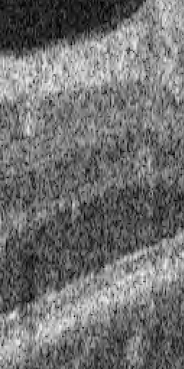
\includegraphics[width=0.18\linewidth]{figures/CirrusPatchExample.png}
	\caption{Example of a patch extracted from a Cirrus OCT volume used in Experiment 1.1. In this patch, while the background is noticeable due to its darker shade, the choroid is harder to be identified by an observer (or a model) due to the lack of context.}
	\label{fig:CirrusPatchExample}
\end{figure}

In Figure \ref{fig:Experiment11Segmentation} it is shown a segmentation performed by the model trained in Run 1 (see Table \ref{tab:Experiment1.1Results}). In this figure it becomes evident that the model learned which areas can be segmented inside the retina, but does not understand how the handle the regions further away. For example, in the area significantly above the retina the background is labeled as SRF. However, the background region closer to the retina is not so frequently labeled as any fluid, since it appears in the patches input to the model. The same problem occurs with the oversegmentation of PED in the choroid region, which does not appear in the input patches significantly.
\par
Oversegmentation beyond the retinal bounds is not exclusive to the Cirrus volumes, as it also appears in the OCT scans from other vendors. This suggests that the issue is primarily due to the small patch size rather than the smaller retinal area captured in Cirrus patches, despite this amplifying the problem. 
\par
In the same figure, it is seen that the model has not learned the anatomical relationships between fluids, since it segmented IRF and PED close to each other. This occurs because the model has not learned the relationship between the retinal landmarks and the fluid types due to the small sized inputs.

\begin{figure}[!ht]
	\centering
	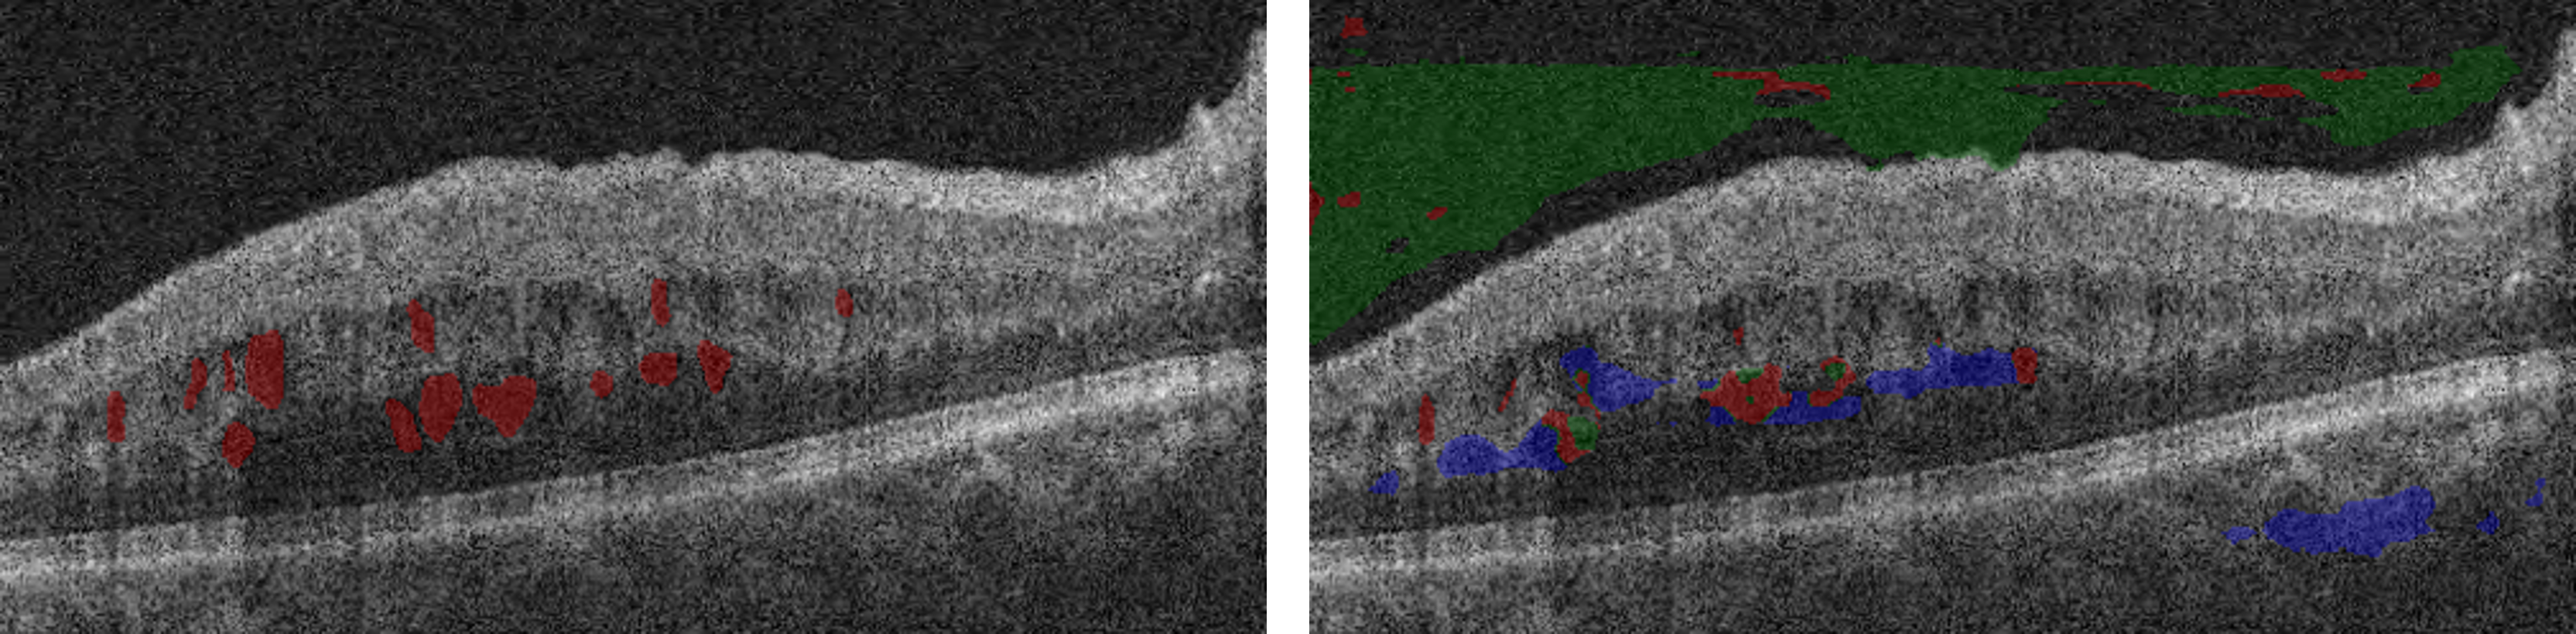
\includegraphics[width=1.0\linewidth]{figures/Experiment11Segmentation.png}
	\caption{Example of a poor segmentation made by the model trained in Run 1 (right). In the left, the GT mask for the same image is shown.}
	\label{fig:Experiment11Segmentation}
\end{figure}

\subsubsection{Experiment 1.2}

The resulting Dice coefficient values obtained in Experiment 1.2, where patches of shape 496 $\times$ 512 were used, are shown in Table \ref{tab:Experiment1.2Results}.

\begin{table*}[!ht]
	\caption{Dice scores for every vendor and fluid for the runs done in Experiment 1.2.}
	\centering
	\resizebox{\textwidth}{!}{\begin{tabular}{|c|c|ccc|ccc|ccc|c|c|c|c|}
		\hline
		% Headers
		\multirow{2}{*}{\textbf{Runs}} & 
		\multirow{2}{*}{\textbf{VF}} & 
		\multicolumn{3}{c|}{\textbf{Cirrus}} & 
		\multicolumn{3}{c|}{\textbf{Spectralis}} & 
		\multicolumn{3}{c|}{\textbf{Topcon}} & 
		\multicolumn{1}{c|}{\multirow{2}{*}{\textbf{IRF}}} & 
		\multirow{2}{*}{\textbf{SRF}} & 
		\multirow{2}{*}{\textbf{PED}} & 
		\multirow{2}{*}{\textbf{Fluid}} \\ \cline{3-11} & &
		\multicolumn{1}{c}{\textbf{IRF}} & 
		\multicolumn{1}{c}{\textbf{SRF}} & 
		\textbf{\textbf{PED}} & 
		\multicolumn{1}{c}{\textbf{IRF}} & 
		\multicolumn{1}{c}{\textbf{SRF}} & 
		\textbf{PED} & 
		\textbf{IRF} & 
		\textbf{SRF} & 
		\textbf{PED} & 
		\multicolumn{1}{c|}{} & & & \\ 
			
		\hline
		
		\textbf{Run 9} & 2 & \multicolumn{1}{c|}{0.291} & \multicolumn{1}{c|}{0.450} & 0.281 & \multicolumn{1}{c|}{0.472} & \multicolumn{1}{c|}{0.638} & 0.394 & \multicolumn{1}{c|}{0.505} & \multicolumn{1}{c|}{0.647} & 0.573 & 0.396 & 0.551 & 0.400 & 0.393 \\

		
		\textbf{Run 10} & 3 & \multicolumn{1}{c|}{\textbf{0.586}} & \multicolumn{1}{c|}{\textbf{0.619}} & \textbf{0.727} & \multicolumn{1}{c|}{0.482} & \multicolumn{1}{c|}{\textbf{0.780}} & \textbf{0.698} & \multicolumn{1}{c|}{\textbf{0.749}} & \multicolumn{1}{c|}{\textbf{0.793}} & \textbf{0.788} & \textbf{0.627} & \textbf{0.711} & \textbf{0.744} & \textbf{0.667} \\

		
		\textbf{Run 11} & 4 & \multicolumn{1}{c|}{0.281} & \multicolumn{1}{c|}{0.453} & 0.415 & \multicolumn{1}{c|}{0.429} & \multicolumn{1}{c|}{0.503} & 0.322 & \multicolumn{1}{c|}{0.228} & \multicolumn{1}{c|}{0.532} & 0.324 & 0.278 & 0.494 & 0.363 & 0.296 \\
		
		\textbf{Run 12} & 0 & \multicolumn{1}{c|}{0.242} & \multicolumn{1}{c|}{0.334} & 0.336 & \multicolumn{1}{c|}{\textbf{0.551}} & \multicolumn{1}{c|}{0.564} & 0.423 & \multicolumn{1}{c|}{0.321} & \multicolumn{1}{c|}{0.643} & 0.407 & 0.325 & 0.488 & 0.377 & 0.339 \\
		
		\hline
		
		\textbf{Set 3} & - & \multicolumn{1}{c|}{0.35} & \multicolumn{1}{c|}{0.46} & 0.44 & \multicolumn{1}{c|}{0.48} & \multicolumn{1}{c|}{0.62} & 0.46 & \multicolumn{1}{c|}{0.45} & \multicolumn{1}{c|}{0.65} & 0.52 & 0.41 & 0.56 & 0.47 & 0.42 \\
		
		\hline
					
	\end{tabular}}
	\label{tab:Experiment1.2Results}
\end{table*}

The information resumed in this table allows the comparison between the performance in models that used smaller patches in Experiment 1.1 with those that used larger patches in this Experiment.
\par
By comparing the ``Set'' rows, it becomes evident an overall increase in performance when using larger patches. In fact, it is observed an increase in almost all the mean values when compared to the best performing set in Experiment 1.1. This increase is larger than one decimal point in some columns, and the largest improvements occur in the volumes obtained using the Cirrus device and when segmenting SRF or PED.
\par
The improvement in performance in Cirrus devices can be explained with the more contextual information given. In Experiment 1.1, the Cirrus patches input to the model were not big enough for the network to capture and understand the retinal borders or the relationship between them and the fluids, thus leading to oversegmentation beyond the retina, as explained. In Experiment 1.2, as the same patch covers the retinal layer and the background simultaneously, the model has learned to not segment beyond the retina. In Figure \ref{fig:BigPatchesSegmentationCirrus}, the B-scan shown in Figure \ref{fig:Experiment11Segmentation}, is segmented by the model trained in Run 9 and it is possible to see that the labeling of the background as fluid is no longer happening.
\par 
This also partially justifies the significant improvement in the SRF and PED Dice coefficient. By providing inputs with enough context, the model is no longer segmenting these fluids outside the retina. However, in Figure \ref{fig:BigPatchesSegmentationCirrus} it is also seen that the model is no longer confusing the fluids in the retina, as it no longer segments the PED close to the IRF. This further justifies that the model is learning the anatomical references associated with PED, as confirmed in Figure \ref{fig:BigPatchesSegmentationTopcon}.
\par
Lastly, it is important to note that the IRF did not improve as much as the other fluids. This happens because the input patches in Experiment 1.1 where extracted mainly from the retina, providing all the anatomical context needed for the IRF segmentation.
\par
In Figure \ref{fig:BigPatchesSegmentationTopcon}, it is seen that the model confuses the choroid with the retina, as it labels parts of that region as IRF and PED. The likely cause for this confusion is that the input patches are often cropped in the middle of the retinal layer (as illustrated in Figure \ref{fig:BigPatchExtraction}), which leads to the model not understanding the position of the choroid relative to the retina. This inaccurate IRF and PED segmentation is probably based on the visual resemblance between the structures seen in the choroid and the fluid pockets in the retina. This indicates that the model does not know the location of the choroid.

\begin{figure}[!ht]
	\centering
	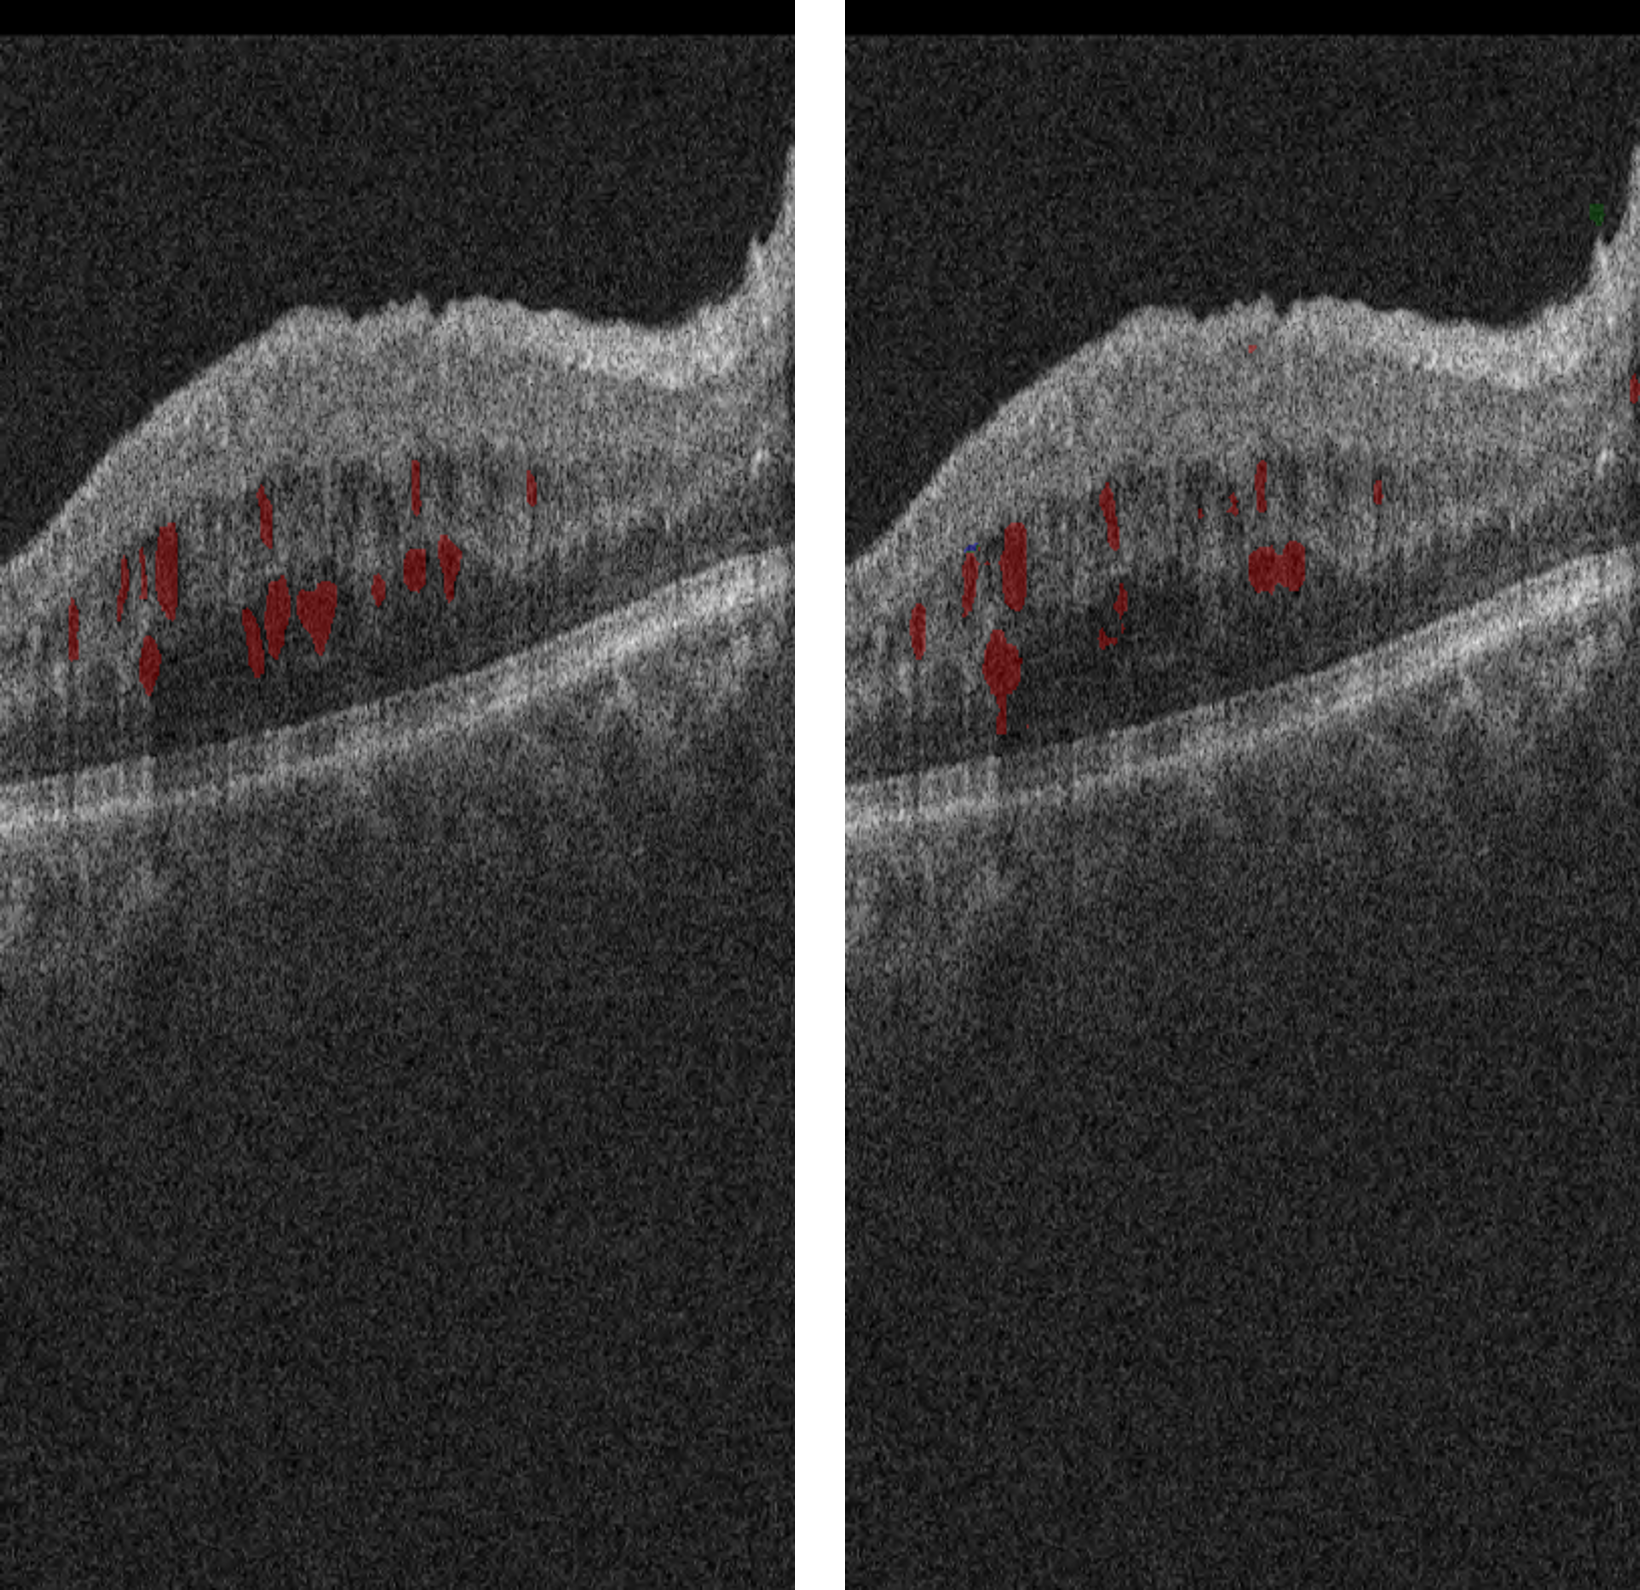
\includegraphics[width=0.5\linewidth]{figures/BigPatchSegmentationCirrus.png}
	\caption{Example of the segmentation done by the model trained in Run 9 (right) and its respective GT mask (left). The B-scan segmented is the same as in Figure \ref{fig:Experiment11Segmentation}.}
	\label{fig:BigPatchesSegmentationCirrus}
\end{figure}

\begin{figure}[!ht]
	\centering
	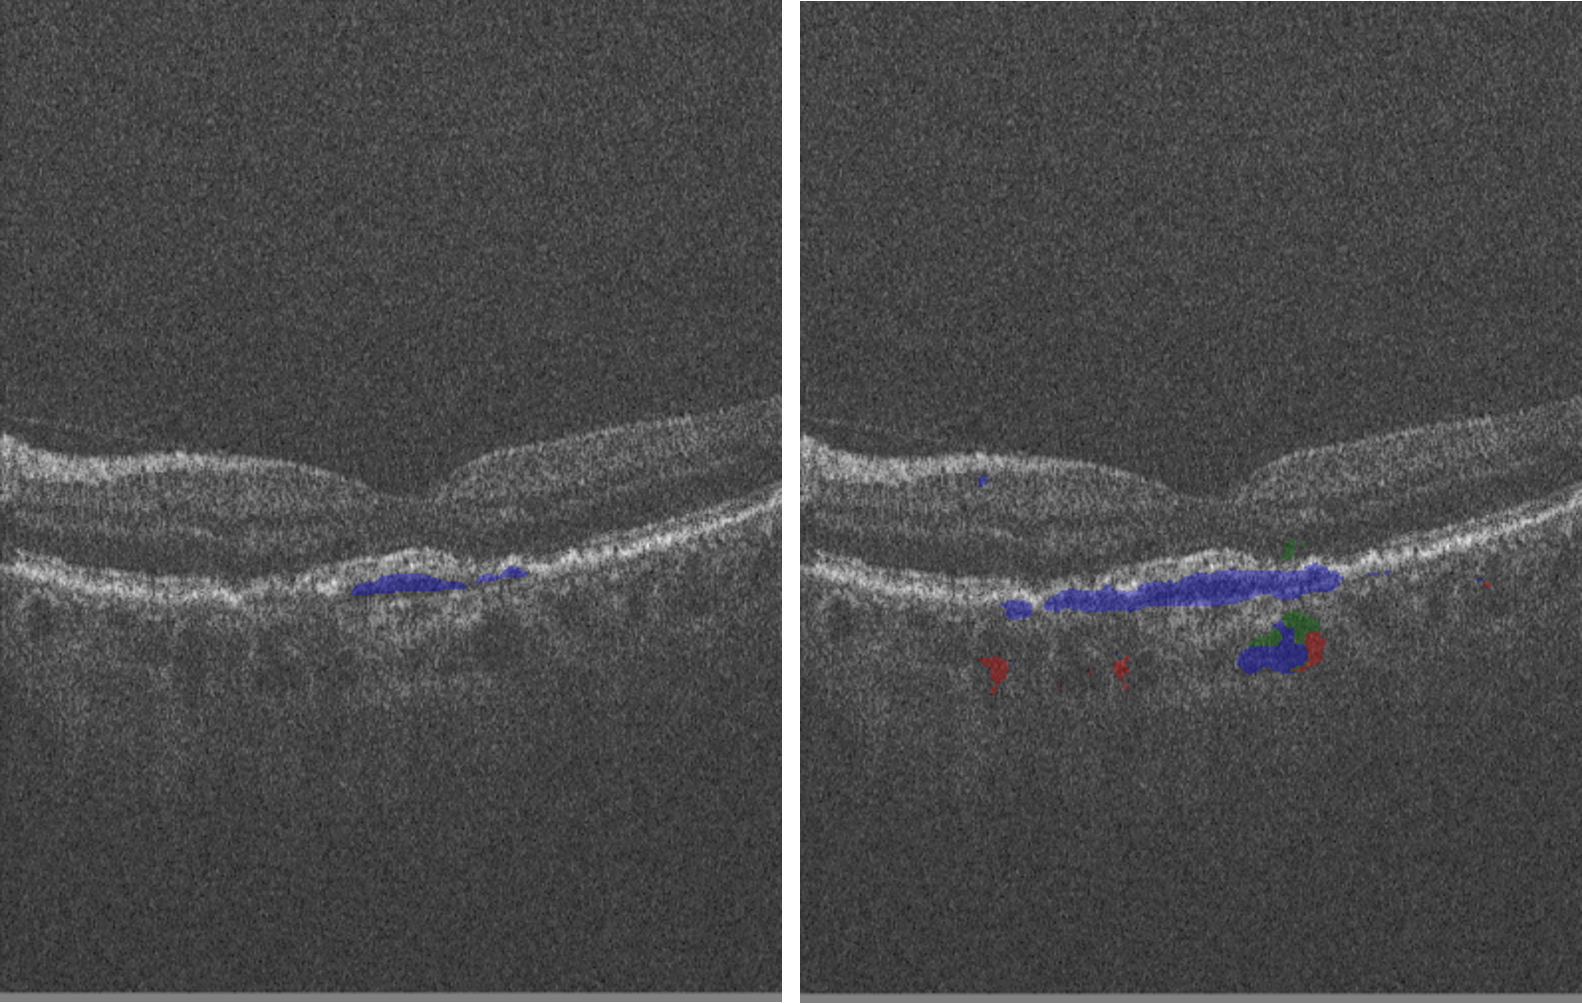
\includegraphics[width=0.6\linewidth]{figures/BigPatchSegmentationTopcon.png}
	\caption{Example of the segmentation done by the model trained in Run 12 (right) and its respective GT mask (left). It is noticeable that the model confuses the choroid with the retina, as segmentation of IRF and PED is performed in the choroid.}
	\label{fig:BigPatchesSegmentationTopcon}
\end{figure}

\subsubsection{Experiment 1.3}
Experiment 1.3 contains all the runs that were performed using vertical patches extracted from resized B-scans as input of the multi-class segmentation U-Net. In the first two sets, shown in Table \ref{tab:Experiment1.3FourPatches}, the models were trained using four vertical patches, obtained as explained in the \ref{Methods} Methods chapter. In this table, the ``Set 4'' is composed of runs that were trained on 100 epochs, while the runs in ``Set 5'' were trained on up to 200 epochs with a 100 epoch patience.

\begin{table*}[!ht]
	\caption{Dice scores for every vendor and fluid for the runs done using four vertical patches extracted from each B-scan. In ``Set 4'', the models were trained in 100 epochs, while in ``Set 5'' the models were trained on up to 200 epochs with a 100 epoch patience. The transformations applied in these sets were the same: horizontal flipping and a maximum rotation of $10^{\circ}$.}
	\centering
	\resizebox{\textwidth}{!}{\begin{tabular}{|c|c|ccc|ccc|ccc|c|c|c|c|}
		\hline
		% Headers
		\multirow{2}{*}{\textbf{Runs}} & 
		\multirow{2}{*}{\textbf{VF}} & 
		\multicolumn{3}{c|}{\textbf{Cirrus}} & 
		\multicolumn{3}{c|}{\textbf{Spectralis}} & 
		\multicolumn{3}{c|}{\textbf{Topcon}} & 
		\multicolumn{1}{c|}{\multirow{2}{*}{\textbf{IRF}}} & 
		\multirow{2}{*}{\textbf{SRF}} & 
		\multirow{2}{*}{\textbf{PED}} & 
		\multirow{2}{*}{\textbf{Fluid}} \\ \cline{3-11} & &
		\multicolumn{1}{c}{\textbf{IRF}} & 
		\multicolumn{1}{c}{\textbf{SRF}} & 
		\textbf{\textbf{PED}} & 
		\multicolumn{1}{c}{\textbf{IRF}} & 
		\multicolumn{1}{c}{\textbf{SRF}} & 
		\textbf{PED} & 
		\textbf{IRF} & 
		\textbf{SRF} & 
		\textbf{PED} & 
		\multicolumn{1}{c|}{} & & & \\ 
			
		\hline
		
		\textbf{Run 13} & 2 & \multicolumn{1}{c|}{0.411} & \multicolumn{1}{c|}{0.665} & 0.498 & \multicolumn{1}{c|}{0.654} & \multicolumn{1}{c|}{0.735} & 0.611 & \multicolumn{1}{c|}{0.731} & \multicolumn{1}{c|}{0.743} & 0.519 & 0.563 & 0.704 & 0.526 & 0.581 \\

		\textbf{Run 14} & 3 & \multicolumn{1}{c|}{0.390} & \multicolumn{1}{c|}{0.520} & 0.217 & \multicolumn{1}{c|}{0.403} & \multicolumn{1}{c|}{0.564} & 0.429 & \multicolumn{1}{c|}{0.378} & \multicolumn{1}{c|}{0.754} & 0.477 & 0.388 & 0.614 & 0.350 & 0.386 \\
		
		\textbf{Run 15} & 4 & \multicolumn{1}{c|}{0.792} & \multicolumn{1}{c|}{\textbf{0.846}} & \textbf{0.883} & \multicolumn{1}{c|}{0.732} & \multicolumn{1}{c|}{\textbf{0.901}} & 0.733 & \multicolumn{1}{c|}{0.615} & \multicolumn{1}{c|}{0.758} & 0.656 & 0.707 & 0.815 & 0.765 & 0.652 \\
		
		\textbf{Run 16} & 0 & \multicolumn{1}{c|}{\textbf{0.810}} & \multicolumn{1}{c|}{0.834} & 0.715 & \multicolumn{1}{c|}{0.779} & \multicolumn{1}{c|}{0.857} & 0.753 & \multicolumn{1}{c|}{0.783} & \multicolumn{1}{c|}{\textbf{0.924}} & \textbf{0.882} & \textbf{0.795} & \textbf{0.871} & \textbf{0.783} & \textbf{0.709} \\
		
		\hline
		
		\textbf{Set 4} & - & \multicolumn{1}{c|}{\textbf{0.60}} & \multicolumn{1}{c|}{\textbf{0.72}} & 0.58 & \multicolumn{1}{c|}{0.64} & \multicolumn{1}{c|}{\textbf{0.76}} & 0.63 & \multicolumn{1}{c|}{0.63} & \multicolumn{1}{c|}{\textbf{0.79}} & 0.63 & 0.61 & \textbf{0.75} & 0.61 & 0.58 \\
		
		\hline
		\hline
		
		\textbf{Run 17} & 2 & \multicolumn{1}{c|}{0.522} & \multicolumn{1}{c|}{0.784} & 0.703 & \multicolumn{1}{c|}{\textbf{0.805}} & \multicolumn{1}{c|}{0.765} & \textbf{0.865} & \multicolumn{1}{c|}{\textbf{0.828}} & \multicolumn{1}{c|}{0.879} & 0.835 & 0.677 & 0.813 & 0.777 & 0.684 \\
	
		\textbf{Run 18} & 3 & \multicolumn{1}{c|}{0.509} & \multicolumn{1}{c|}{0.654} & 0.598 & \multicolumn{1}{c|}{0.590} & \multicolumn{1}{c|}{0.806} & 0.755 & \multicolumn{1}{c|}{0.777} & \multicolumn{1}{c|}{0.787} & 0.792 & 0.621 & 0.729 & 0.697 & 0.622 \\
					
		\textbf{Run 19} & 4 & \multicolumn{1}{c|}{0.377} & \multicolumn{1}{c|}{0.387} & 0.398 & \multicolumn{1}{c|}{0.478} & \multicolumn{1}{c|}{0.624} & 0.398 & \multicolumn{1}{c|}{0.483} & \multicolumn{1}{c|}{0.729} & 0.448 & 0.436 & 0.567 & 0.420 & 0.399 \\
		
		\textbf{Run 20} & 0 & \multicolumn{1}{c|}{0.753} & \multicolumn{1}{c|}{0.697} & 0.696 & \multicolumn{1}{c|}{0.779} & \multicolumn{1}{c|}{0.844} & 0.783 & \multicolumn{1}{c|}{0.691} & \multicolumn{1}{c|}{0.720} & 0.671 & 0.735 & 0.731 & 0.702 & 0.637 \\
		
		\hline
		
		\textbf{Set 5} & - & \multicolumn{1}{c|}{0.54} & \multicolumn{1}{c|}{0.63} & \textbf{0.60} & \multicolumn{1}{c|}{\textbf{0.66}} & \multicolumn{1}{c|}{0.76} & \textbf{0.70} & \multicolumn{1}{c|}{\textbf{0.69}} & \multicolumn{1}{c|}{0.78} & \textbf{0.69} & \textbf{0.62} & 0.71 & \textbf{0.65} & \textbf{0.59} \\
		
		\hline
			
	\end{tabular}}
	\label{tab:Experiment1.3FourPatches}
\end{table*}

The results of the sets shown in Table \ref{tab:Experiment1.3FourPatches} can be compared within each other and to the results obtained in the sets of previous experiments. 
\par
When comparing the results between sets, it is noticeable that the runs with the best scores are mostly located in the ``Set'' that trained less epochs. For, the model validated on fold 4 (Run 15) sees a significant decrease in performance when trained for 100 more epochs (Run 19). When looking at the models validation loss per epoch, the lowest value is attained commonly before the 100 epochs. Since the model that is saved in each run is the model that attains the lowest loss on validation data, this means that the models trained in 100 or 200 epochs should perform equally, as long as the lowest validation loss occurred prior to the 100 epoch mark.
\par
However, looking at Figure \ref{fig:TrainingValidationLosses}, where the training and validation loss curves for the Run 13 and Run 17 are shown, similar trends and behavior is seen in both models. This does not reflect to similar performances in the same validation data, as shown in Table \ref{tab:Experiment1.3FourPatches}. In fact, a substantial increment is seen in Run 17.
\par
To justify this behavior, it is important to remind that the training of a neural network has some randomness associated with it. One aspect that affects the model performance despite using the same data and architecture is the weight initialization. The random initialization of weights affects the trajectory of gradient descent, resulting in different convergences for different runs. Another factor that affects the model learning is the data that composes each batch. The images that form a batch are randomly fetch from the available input images. This create batches with different distributions of characteristics, affecting the model's view of the data. Data augmentation, which randomly selects images to apply the transformations as they are fetch, also influences the model performance. Lastly, there are other factors that have a much smaller impact such as the optimizer behavior and non-deterministic operations at the GPU level \parencite{Akesson2024, Altarabichi2024}. 
\par
In Appendix \ref{ap1:SegmentationUNetVariability}, Table \ref{tab:SegmentationUNetVariability} shows the results for multiple models that were trained on the same conditions, aiming to give an insight on how the randomness associated with the U-Net affects the models performances. Five models were validated on fold 2, while nine models were validated in fold 3. The results obtained corroborate the differences seen in Table \ref{tab:Experiment1.3FourPatches}, where models trained on the same conditions for more epochs can obtain significantly worse Dice scores in validation.

\begin{figure}[!ht]
	\centering
	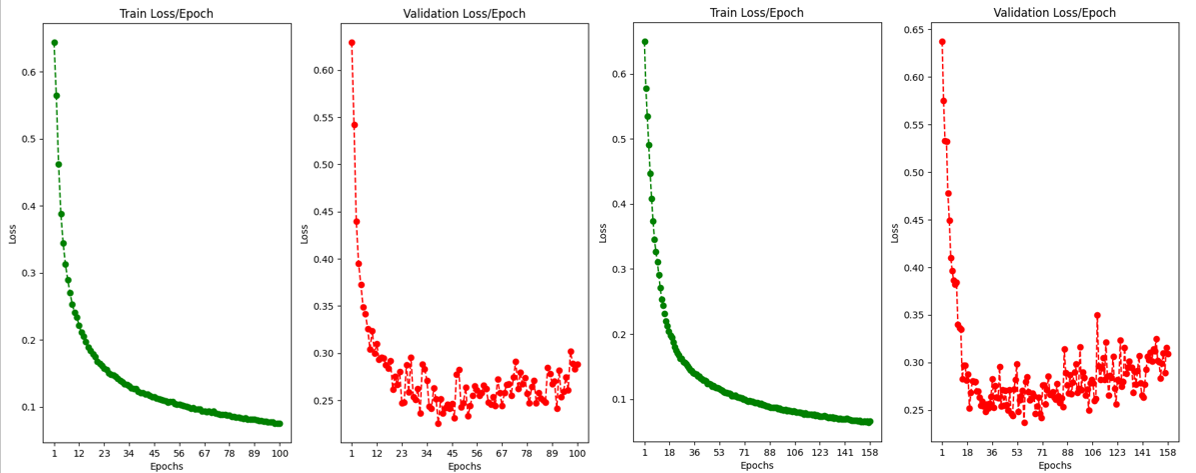
\includegraphics[width=1.0\linewidth]{figures/TrainingValidationLosses.png}
	\caption{Training and validation losses in Run 13 (left) and Run 17 (right). Despite reaching the validation loss minimum in a similar number of epochs and having comparable training and validation loss curves, the performance is really different in Table \ref{tab:Experiment1.3FourPatches}.}
	\label{fig:TrainingValidationLosses}
\end{figure}

Despite the differences in the results shown in Table \ref{tab:Experiment1.3FourPatches}, both sets attained better performances than the best results in the previous experiments. The improvements were significant, registering increases above 0.2 in some metrics when compared with the results in Experiment 1.3. Every vendor and every fluid seen a considerable increase of performance.
\par
This overall increment can be attributed to two changes: training on vertical patches and resizing the images. By training the models on vertical patches, the model can focus on the finer details within each region. This is important because the retinal fluid segmentation relies heavily on the retina's characteristics, a region that occupies a small portion of the image. Despite the input being smaller than in Experiment 1.3, the patches could still capture the transitions between the retina and the choroid or background. Since the input size is smaller, less storage it occupies in memory, therefore allowing an increase in the batch size, that translates to a faster and more stable convergence. Meanwhile, the image's resizing makes the inputs more homogeneous across different vendors. This results in the same structures being represented with consistent shapes and sizes across the B-scans from different vendors, resulting in a significantly simpler learning process.
\par
It was seen in Figure \ref{fig:BigPatchesSegmentationTopcon} that the model predicted fluid masks in the choroid region. In Figure \ref{fig:VerticalPatchesSegmentationTopcon}, it is seen that the models trained on vertical patches no longer predict fluid in the choroid region, despite inferring on the same B-scan. This means that, by feeding vertical patches to the model, it learns to not segment below the retina, in the choroid. This was not previously understood by the model when big patches were input, since these would frequently not capture both the retinal layer and the choroid in the same patch, restraining the model from learning the relative position of the choroid and its relationship with the fluid prediction.

\begin{figure}[!ht]
	\centering
	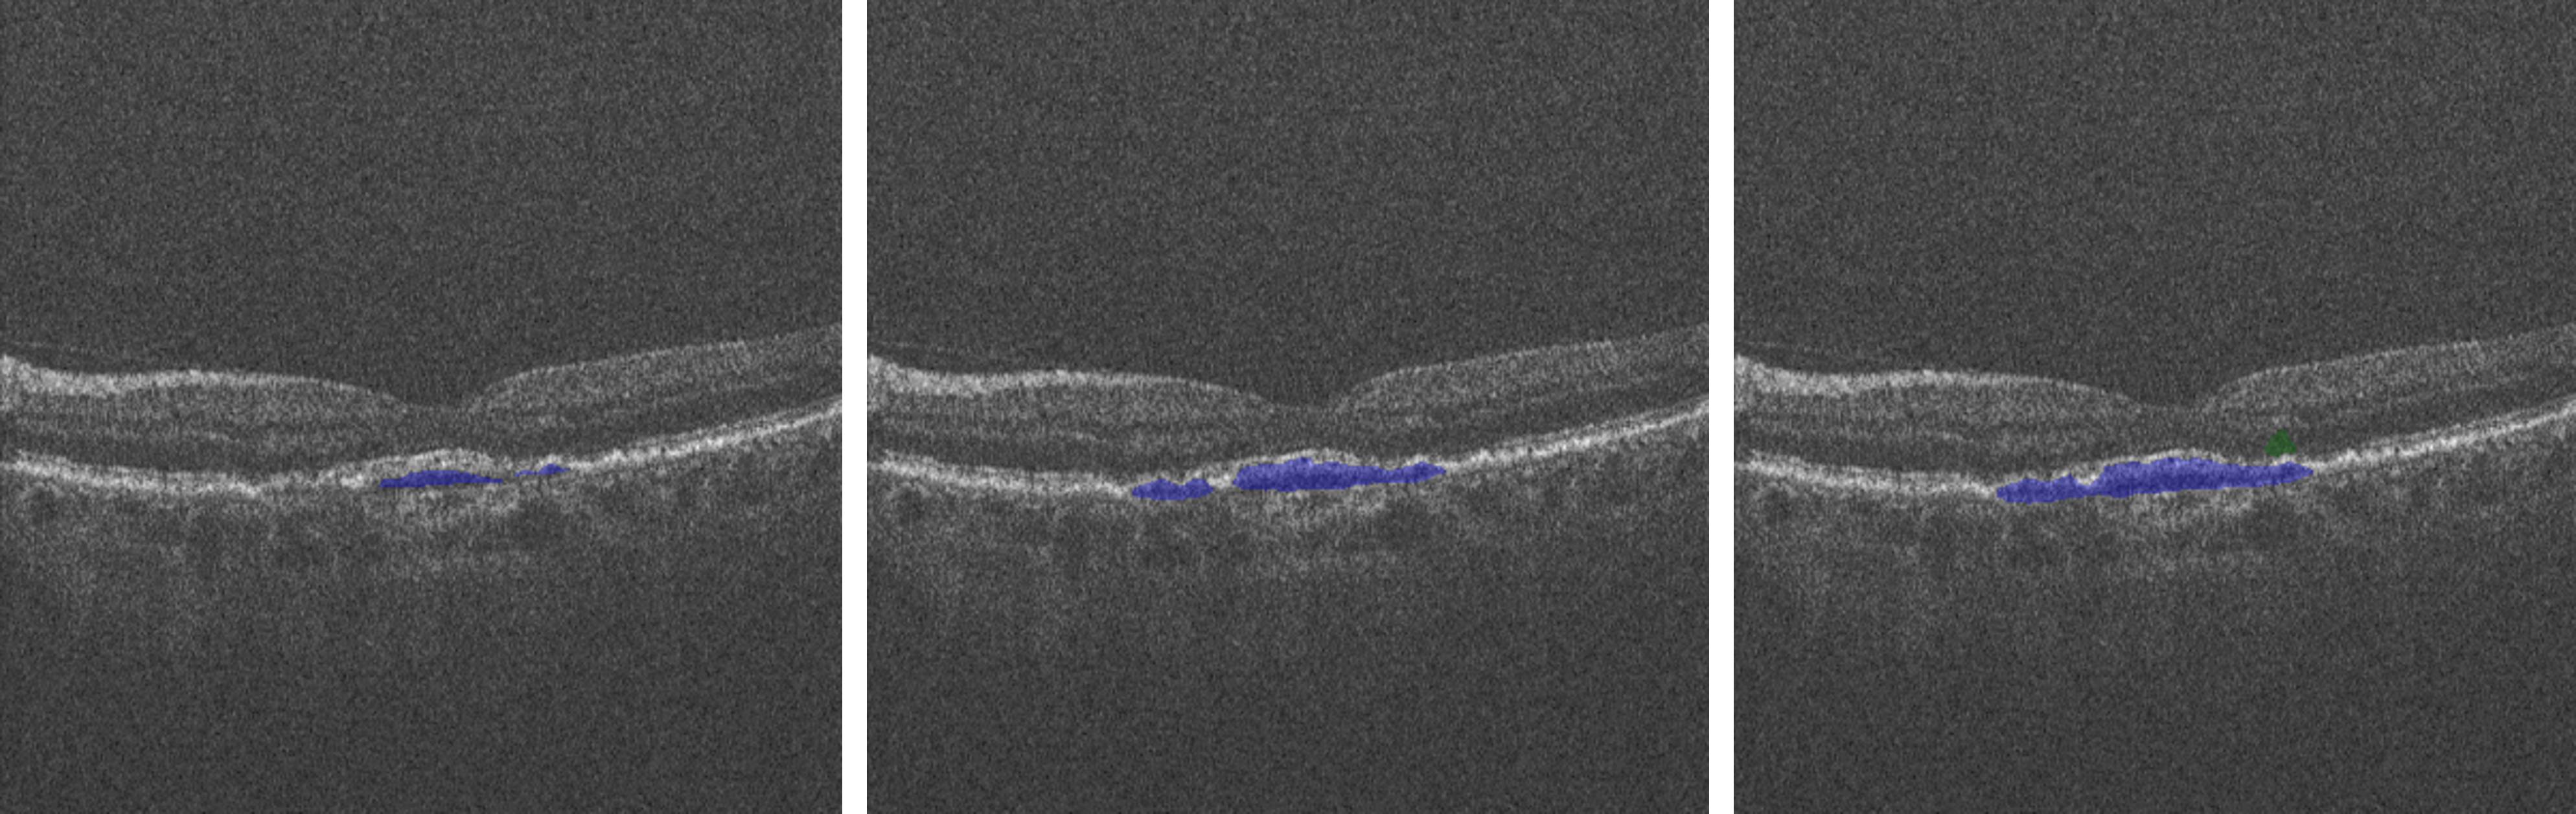
\includegraphics[width=1.0\linewidth]{figures/VerticalPatchesSegmentationTopcon.png}
	\caption{Predicted masks by the models trained on Run 16 (middle) and Run 20 (right) and their respective GT (left).}
	\label{fig:VerticalPatchesSegmentationTopcon}
\end{figure}

Afterwards, the use of seven and thirteen patches extracted from each B-scan was tested and the results are shown in Table \ref{tab:Experiment1.3SevenVsThirteenPatches}. Two models were trained for each number of patches extracted, one validated on fold 2 and another validated on fold 3. The models were trained on 200 maximum epochs, with a 25 epoch patience applied after the first 100 epochs.

\begin{table*}[!ht]
	\caption{Dice scores for every vendor and fluid for the runs done using seven (Runs 21 and 22) and thirteen (Runs 23 and 24) vertical patches extracted from each B-scan. Only two folds were used in order to understand the viability of using these numbers of patches, which is represented in the column ``P''. Runs 17 and 18 are shown here to make the comparison between the number of patches easier. The values shown in bold represent the best value for the models trained with the same number of patches.}
	\centering
	\resizebox{\textwidth}{!}{\begin{tabular}{|c|c|c|ccc|ccc|ccc|c|c|c|c|}
		\hline
		% Headers
		\multirow{2}{*}{\textbf{Runs}} & 
		\multirow{2}{*}{\textbf{VF}} & 
		\multirow{2}{*}{\textbf{P}} &
		\multicolumn{3}{c|}{\textbf{Cirrus}} & 
		\multicolumn{3}{c|}{\textbf{Spectralis}} & 
		\multicolumn{3}{c|}{\textbf{Topcon}} & 
		\multicolumn{1}{c|}{\multirow{2}{*}{\textbf{IRF}}} & 
		\multirow{2}{*}{\textbf{SRF}} & 
		\multirow{2}{*}{\textbf{PED}} & 
		\multirow{2}{*}{\textbf{Fluid}} \\ \cline{4-12} & & &
		\multicolumn{1}{c}{\textbf{IRF}} & 
		\multicolumn{1}{c}{\textbf{SRF}} & 
		\textbf{\textbf{PED}} & 
		\multicolumn{1}{c}{\textbf{IRF}} & 
		\multicolumn{1}{c}{\textbf{SRF}} & 
		\textbf{PED} & 
		\textbf{IRF} & 
		\textbf{SRF} & 
		\textbf{PED} & 
		\multicolumn{1}{c|}{} & & & \\ 
		
		\hline
			
		\textbf{Run 17} & 2 & 4 & \multicolumn{1}{c|}{0.522} & \multicolumn{1}{c|}{0.784} & \textbf{0.703} & \multicolumn{1}{c|}{\textbf{0.805}} & \multicolumn{1}{c|}{0.765} & \textbf{0.865} & \multicolumn{1}{c|}{0.828} & \multicolumn{1}{c|}{0.879} & 0.835 & 0.677 & 0.813 & \textbf{0.777} & 0.684 \\
		
		\textbf{Run 21} & 2 & 7 & \multicolumn{1}{c|}{\textbf{0.556}} & \multicolumn{1}{c|}{\textbf{0.837}} & 0.672 & \multicolumn{1}{c|}{0.761} & \multicolumn{1}{c|}{\textbf{0.853}} & 0.848 & \multicolumn{1}{c|}{\textbf{0.829}} & \multicolumn{1}{c|}{0.908} & \textbf{0.858} & \textbf{0.685} & \textbf{0.864} & 0.767 & \textbf{0.681} \\
		
		\textbf{Run 23} & 2 & 13 & \multicolumn{1}{c|}{0.500} & \multicolumn{1}{c|}{0.762} & 0.635 & \multicolumn{1}{c|}{0.672} & \multicolumn{1}{c|}{0.790} & 0.773 & \multicolumn{1}{c|}{0.819} & \multicolumn{1}{c|}{\textbf{0.936}} & 0.805 & 0.639 & 0.826 & 0.718 & 0.637 \\
		
		\hline
		\hline
		
		\textbf{Run 18} & 3 & 4 & \multicolumn{1}{c|}{0.509} & \multicolumn{1}{c|}{0.654} & 0.598 & \multicolumn{1}{c|}{0.590} & \multicolumn{1}{c|}{0.806} & \textbf{0.755} & \multicolumn{1}{c|}{\textbf{0.777}} & \multicolumn{1}{c|}{\textbf{0.787}} & \textbf{0.792} & 0.621 & 0.729 & 0.697 & 0.622 \\
		
		\textbf{Run 22} & 3 & 7 & \multicolumn{1}{c|}{\textbf{0.734}} & \multicolumn{1}{c|}{\textbf{0.855}} & 0.836 & \multicolumn{1}{c|}{\textbf{0.636}} & \multicolumn{1}{c|}{\textbf{0.846}} & 0.689 & \multicolumn{1}{c|}{0.686} & \multicolumn{1}{c|}{0.781} & 0.731 & \textbf{0.700} & \textbf{0.822} & \textbf{0.771} & \textbf{0.672} \\
		
		\textbf{Run 24} & 3 & 13 & \multicolumn{1}{c|}{0.612} & \multicolumn{1}{c|}{0.648} & \textbf{0.882} & \multicolumn{1}{c|}{0.455} & \multicolumn{1}{c|}{0.636} & 0.548 & \multicolumn{1}{c|}{0.499} & \multicolumn{1}{c|}{0.593} & 0.668 & 0.542 & 0.622 & 0.745 & 0.536 \\
		
		\hline
			
	\end{tabular}}
	\label{tab:Experiment1.3SevenVsThirteenPatches}
\end{table*}

Training the models on more patches per B-scan, significantly increases the quantity of data that is seen by the model during an epoch. Therefore, each epoch takes much longer to complete, requiring more computation power, leading to often bottlenecks. However, since the model sees many more patches per epoch, the model reaches the validation loss minimum much earlier than in the models trained with four patches. 
\par
In Figure \ref{fig:ValidationLossesFourSevenThirteenPatches}, it is possible to see a comparison between the training and validation losses of the models validated on fold 2, using four, seven, and thirteen vertical patches per B-scan. Despite following the same trends, the model learns significantly faster as the number of patches increases, resulting in a faster progression of the validation loss. As a result the models starts to overfit much earlier and aggressively with larger number of patches, which is signaled by the increase in validation loss after reaching low values.

\begin{figure}[!ht]
	\centering
	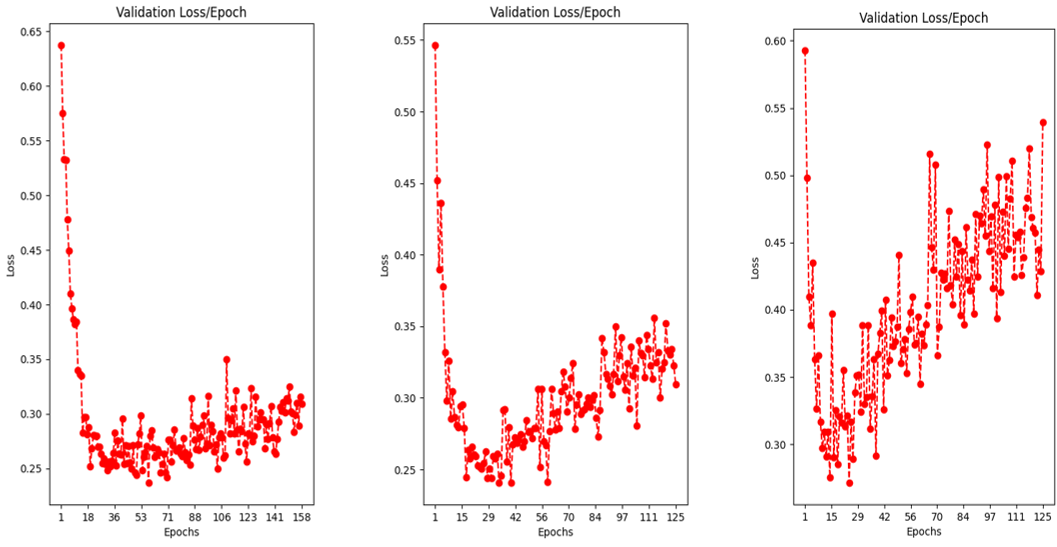
\includegraphics[width=1.0\linewidth]{figures/ValidationLossesFourSevenThirteenPatches.png}
	\caption{Training and validation losses for models validated on fold 2. The curves on the left are from the model trained on Run 17 with four patches, while the middle curves are from the model trained on Run 21, with seven patches. The curves on the right are from the model trained on Run 23, with thirteen patches.}
	\label{fig:ValidationLossesFourSevenThirteenPatches}
\end{figure}

When comparing the models' performances, by looking at Table \ref{tab:Experiment1.3FourPatches}, the models trained on thirteen patches are outperformed by those trained in fewer patches. These results suggest that the faster progression in validation loss for the model trained with thirteen patches inhibits its ability to converge to a solution as optimal as those achieved by models trained more slowly with fewer patches.
\par
The performance differences between the models trained with four and seven patches are less pronounced than those when either is compared to the model trained with thirteen patches. However, the model trained with seven patches consistently outperforms the one trained with four in most metrics. In the few cases the model trained with four patches performs better, the other model still achieves comparable results. The reverse is not true: when the model trained with seven patches outperforms the model trained with four patches, the performance gap is significantly larger. For these reasons, the model trained with seven patches was considered superior.
\par
Nevertheless, both models still make wrongful predictions, which do not respect the anatomic context of the image. For example, in Figure \ref{fig:CirrusSegmentationErrors}, the IRF fluid is predicted below the PED, which is not anatomically possible and there are no examples in the dataset that exhibit this relationship.
\par
While this unexpected behavior could be attributed to the B-scan differing from the examples seen in training, the subsequent runs aimed to investigate whether this was caused by the rotation transformation. It was hypothesized that random rotations could alter the vertical order of fluid regions, potentially leading the model to learn incorrect patterns. Additionally, the padding that is performed to fill the rotated areas, as illustrated in Figure \ref{fig:TransformationsInVerticalPatches}, could also influence the model's performance.

\begin{figure}[!ht]
	\centering
	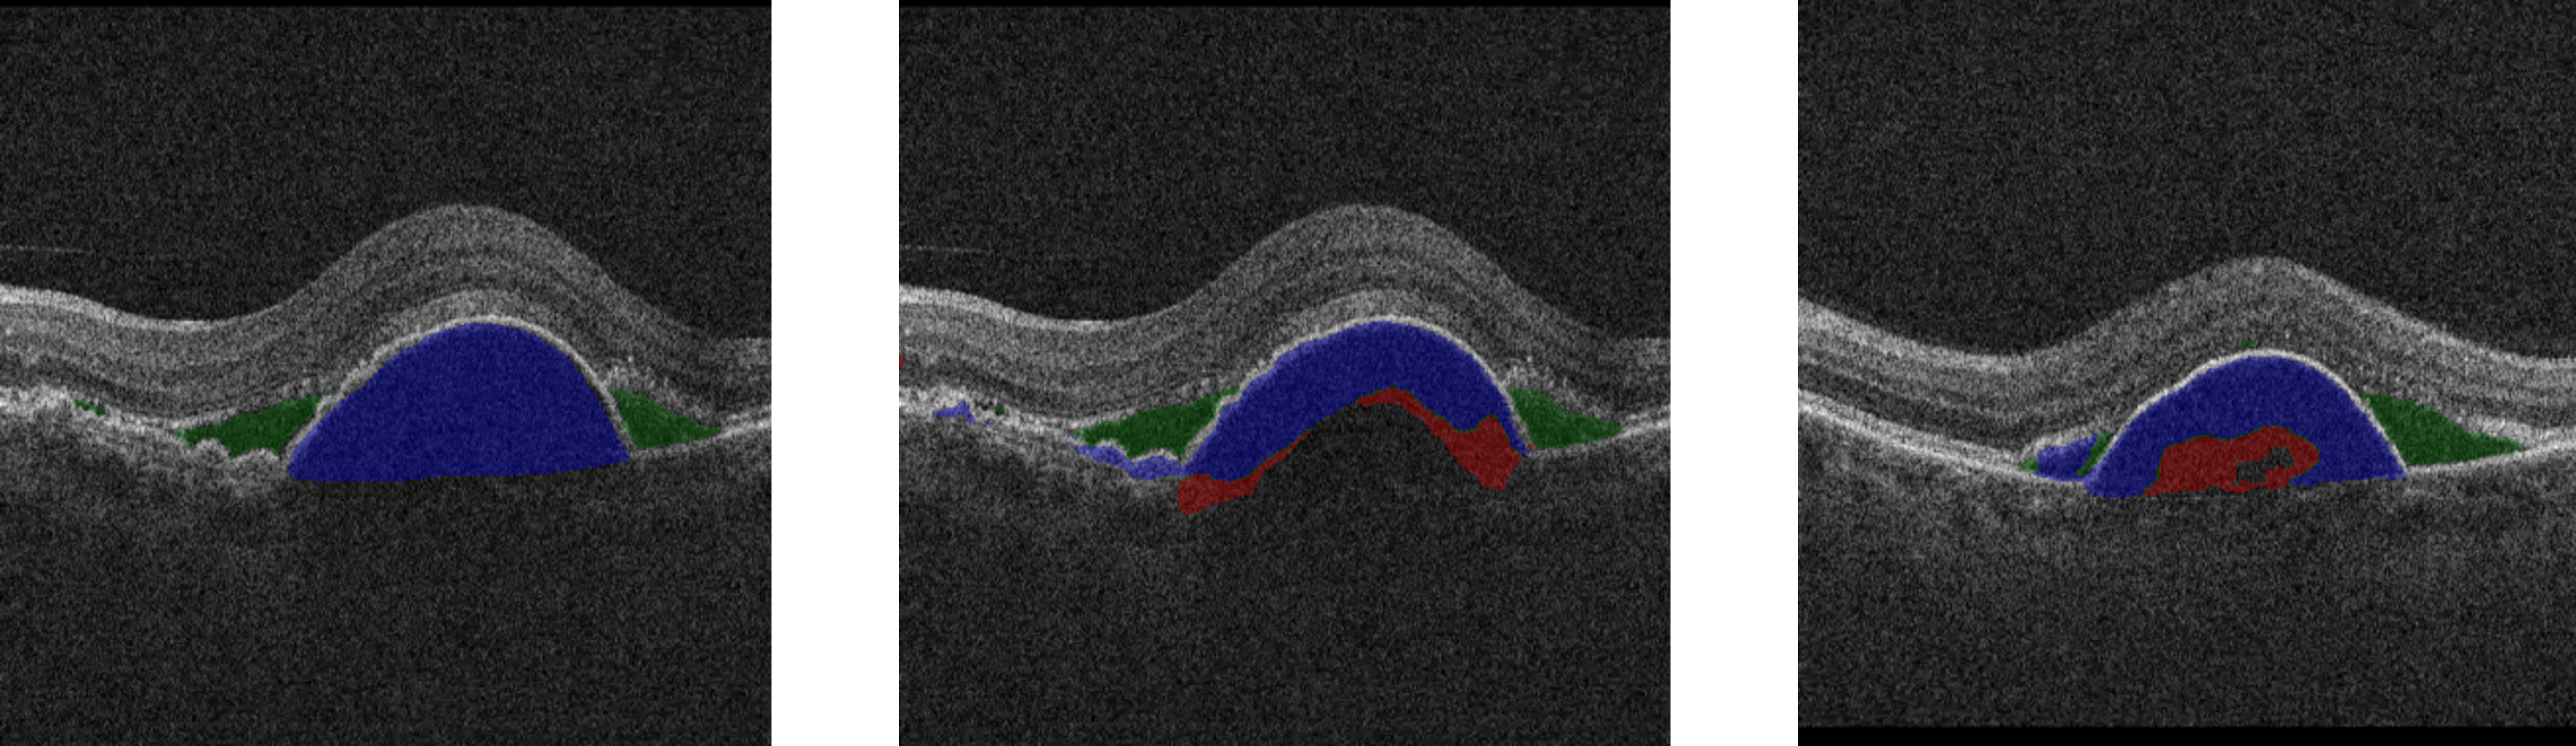
\includegraphics[width=1.0\linewidth]{figures/CirrusSegmentationErrors.png}
	\caption{Segmentation errors in Cirrus B-scans. The GT fluid masks, seen on the left, show a large region of PED fluid. Meanwhile, the predictions made by the models trained in Run 21 and 23, which respectively correspond to the B-scans in the middle and right, classify the center of this region as IRF.}
	\label{fig:CirrusSegmentationErrors}
\end{figure}

\begin{figure}[!ht]
	\centering
	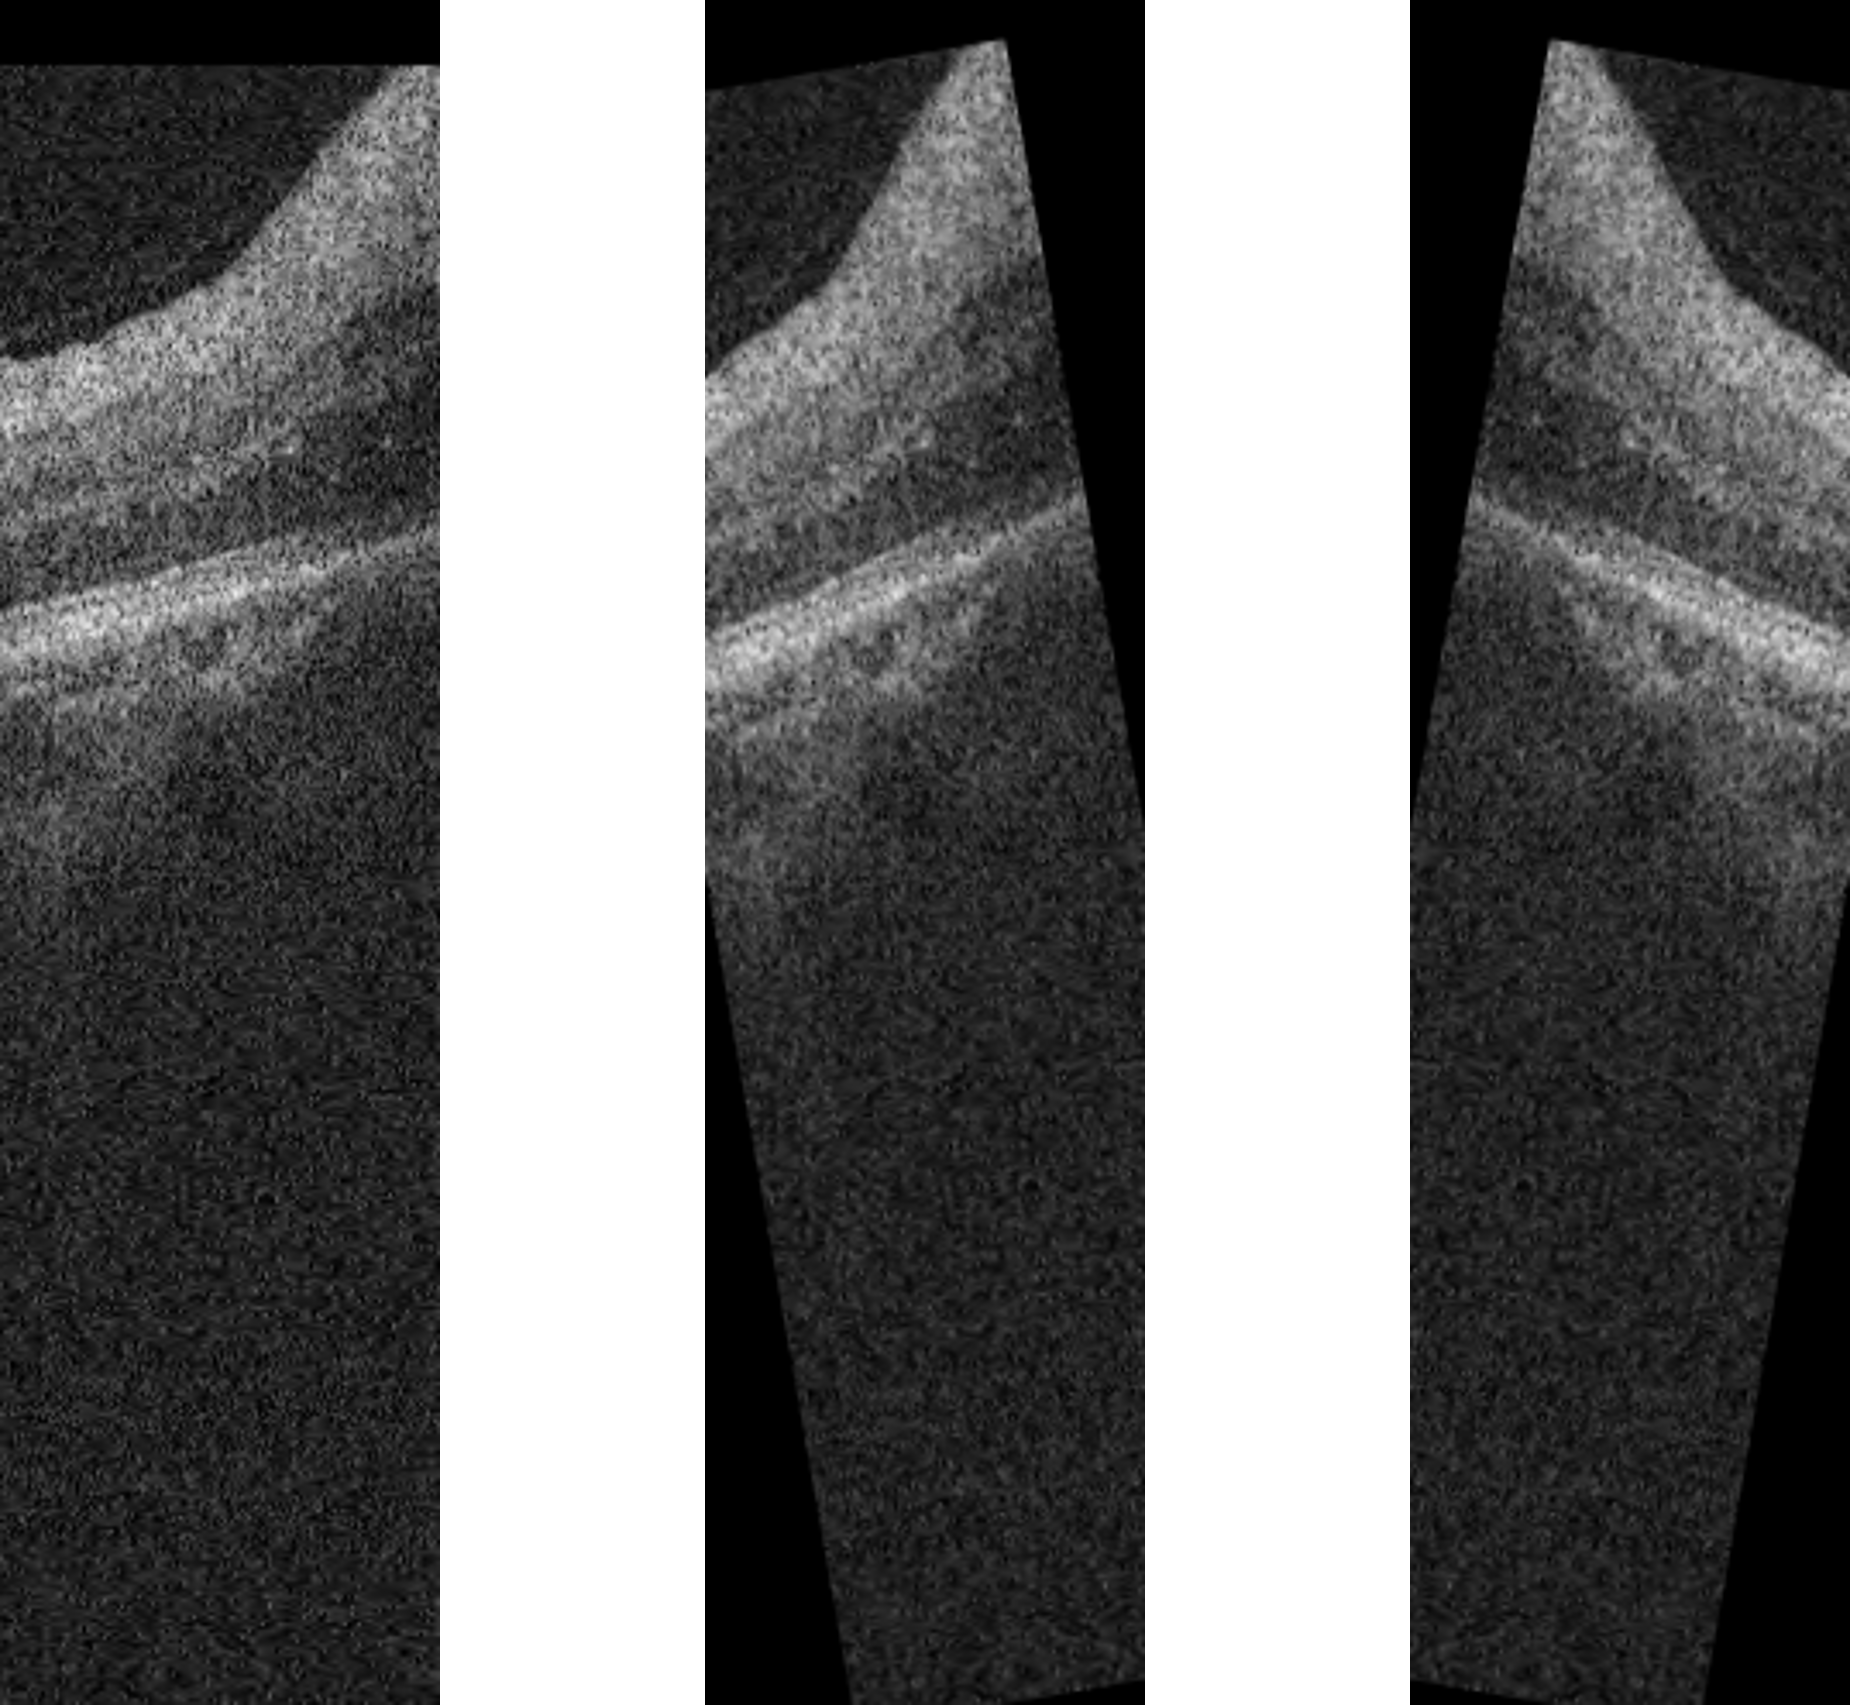
\includegraphics[width=0.5\linewidth]{figures/TransformationsInVerticalPatches.png}
	\caption{Transformations applied to a vertical patch of a Cirrus B-scan. The original vertical patch (left) can be rotated a maximum of $10^{\circ}$, a transformation that is shown in the middle image. The image on the right represents the combination of a $10^{\circ}$ rotation and an horizontal flip. It is seen that the rotation transform pads a significant portion of the image, reducing the information in the input.}
	\label{fig:TransformationsInVerticalPatches}
\end{figure}

Table \ref{tab:Experiment1.3SevenPatchesNoRotation} shows the results obtained in the runs performed using only horizontal flipping as transformation, without performing rotations. In these runs, seven input patches were extracted from each B-scan. Due to the faster progression of the models trained using seven vertical patches per B-scan, the model was trained on a minimum of 25 epochs with a 25 epoch patience after. Since the validation minimum is usually attained early in the models trained with more patches, as seen in Figure \ref{fig:ValidationLossesFourSevenThirteenPatches}, by setting such early stopping, the training would be much faster while maintaining the same performance.

\begin{table*}[!ht]
	\caption{Dice scores for every vendor and fluid using seven vertical patches. The only transformation performed in these runs was horizontal flipping, without rotation. Runs 21 and 22 are also shown, promoting an easier comparison.}
	\centering
	\resizebox{\textwidth}{!}{\begin{tabular}{|c|c|ccc|ccc|ccc|c|c|c|c|}
			\hline
			% Headers
			\multirow{2}{*}{\textbf{Runs}} & 
			\multirow{2}{*}{\textbf{VF}} & 
			\multicolumn{3}{c|}{\textbf{Cirrus}} & 
			\multicolumn{3}{c|}{\textbf{Spectralis}} & 
			\multicolumn{3}{c|}{\textbf{Topcon}} & 
			\multicolumn{1}{c|}{\multirow{2}{*}{\textbf{IRF}}} & 
			\multirow{2}{*}{\textbf{SRF}} & 
			\multirow{2}{*}{\textbf{PED}} & 
			\multirow{2}{*}{\textbf{Fluid}} \\ \cline{3-11} & &
			\multicolumn{1}{c}{\textbf{IRF}} & 
			\multicolumn{1}{c}{\textbf{SRF}} & 
			\textbf{\textbf{PED}} & 
			\multicolumn{1}{c}{\textbf{IRF}} & 
			\multicolumn{1}{c}{\textbf{SRF}} & 
			\textbf{PED} & 
			\textbf{IRF} & 
			\textbf{SRF} & 
			\textbf{PED} & 
			\multicolumn{1}{c|}{} & & & \\ 
			
			\hline
			
			\textbf{Run 25} & 2 & \multicolumn{1}{c|}{0.406} & \multicolumn{1}{c|}{0.789} & 0.656 & \multicolumn{1}{c|}{0.595} & \multicolumn{1}{c|}{\textbf{0.805}} & \textbf{0.786} & \multicolumn{1}{c|}{0.762} & \multicolumn{1}{c|}{0.841} & 0.797 & 0.560 & 0.809 & 0.727 & 0.620 \\

			
			\textbf{Run 26} & 3 & \multicolumn{1}{c|}{0.589} & \multicolumn{1}{c|}{0.775} & 0.553 & \multicolumn{1}{c|}{0.586} & \multicolumn{1}{c|}{0.803} & 0.766 & \multicolumn{1}{c|}{0.769} & \multicolumn{1}{c|}{\textbf{0.827}} & 0.755 & 0.654 & 0.799 & 0.664 & 0.617 \\
			
			
			\textbf{Run 27} & 4 & \multicolumn{1}{c|}{\textbf{0.797}} & \multicolumn{1}{c|}{\textbf{0.845}} & \textbf{0.827} & \multicolumn{1}{c|}{\textbf{0.734}} & \multicolumn{1}{c|}{0.782} & 0.659 & \multicolumn{1}{c|}{0.533} & \multicolumn{1}{c|}{0.756} & 0.553 & 0.674 & 0.798 & 0.686 & 0.626 \\
			
			
			\textbf{Run 28} & 0 & \multicolumn{1}{c|}{0.677} & \multicolumn{1}{c|}{0.842} & 0.699 & \multicolumn{1}{c|}{0.681} & \multicolumn{1}{c|}{0.799} & 0.732 & \multicolumn{1}{c|}{\textbf{0.791}} & \multicolumn{1}{c|}{0.846} & \textbf{0.854} & \textbf{0.719} & \textbf{0.836} & \textbf{0.762} & \textbf{0.665} \\
			
			
			\hline
			
			\textbf{Set 6} & - & \multicolumn{1}{c|}{0.62} & \multicolumn{1}{c|}{0.81} & 0.68 & \multicolumn{1}{c|}{0.65} & \multicolumn{1}{c|}{0.80} & 0.74 & \multicolumn{1}{c|}{0.71} & \multicolumn{1}{c|}{0.82} & 0.74 & 0.65 & 0.81 & 0.71 & 0.63 \\
			
			\hline
			\hline
			
			\textbf{Run 21} & 2 & \multicolumn{1}{c|}{0.556} & \multicolumn{1}{c|}{0.837} & 0.672 & \multicolumn{1}{c|}{0.761} & \multicolumn{1}{c|}{0.853} & 0.848 & \multicolumn{1}{c|}{0.829} & \multicolumn{1}{c|}{0.908} & 0.858 & 0.685 & 0.864 & 0.767 & 0.681 \\
			
			\textbf{Run 22} & 3 & \multicolumn{1}{c|}{0.734} & \multicolumn{1}{c|}{0.855} & 0.836 & \multicolumn{1}{c|}{0.636} & \multicolumn{1}{c|}{0.846} & 0.689 & \multicolumn{1}{c|}{0.686} & \multicolumn{1}{c|}{0.781} & 0.731 & 0.700 & 0.822 & 0.771 & 0.672 \\
			
			\hline
			
	\end{tabular}}
	\label{tab:Experiment1.3SevenPatchesNoRotation}
\end{table*}

Removing the rotation from the transformations applied to the input data, significantly worsen the models performances. In Table \ref{tab:Experiment1.3SevenPatchesNoRotation}, when comparing Run 21 to Run 25, which were validated on the same fold, the model trained in Run 21, in which rotation was applied, outperformed the model trained in Run 25 in every single metric. Following the same trend, the model trained in Run 26 only outperformed the model trained in Run 22 in four metrics: Spectralis PED and all the fluids in Topcon.
\par
The differences in performance here exposed highlight the importance of applying transformations to the inputs, despite the mentioned loss of information associated with it. The introduction of variability to the input data significantly improved the model's generalization, preventing the model from overfitting so early on the training stage. In OCT, the rotation is particularly important since different images exhibit different orientations of the retinal layer. By introducing rotation to the inputs, the model becomes more robust to varied input data and less specific to the orientations seen in training. This transformation particularly enhances the performance of the models trained in B-scans where the retinal layer appears horizontal. In Figure \ref{fig:DifferentRetinaOrientation}, two B-scans that illustrate the variability of the retina orientation are shown.
\par
Nevertheless, the lack of rotation in the training dataset mitigated the poor segmentation shown in Figure \ref{fig:CirrusSegmentationErrors}. As exhibited in Figure \ref{fig:SegmentationErrorsNoRotation}, the model that was trained without rotation does not predict as much IRF in the PED region as those trained with rotation, as shown in Figure \ref{fig:CirrusSegmentationErrors}. However, the model that was trained without rotation also predicted IRF in a region that none of the other models did, exemplifying why this model performed worse than those.

\begin{figure}[!ht]
	\centering
	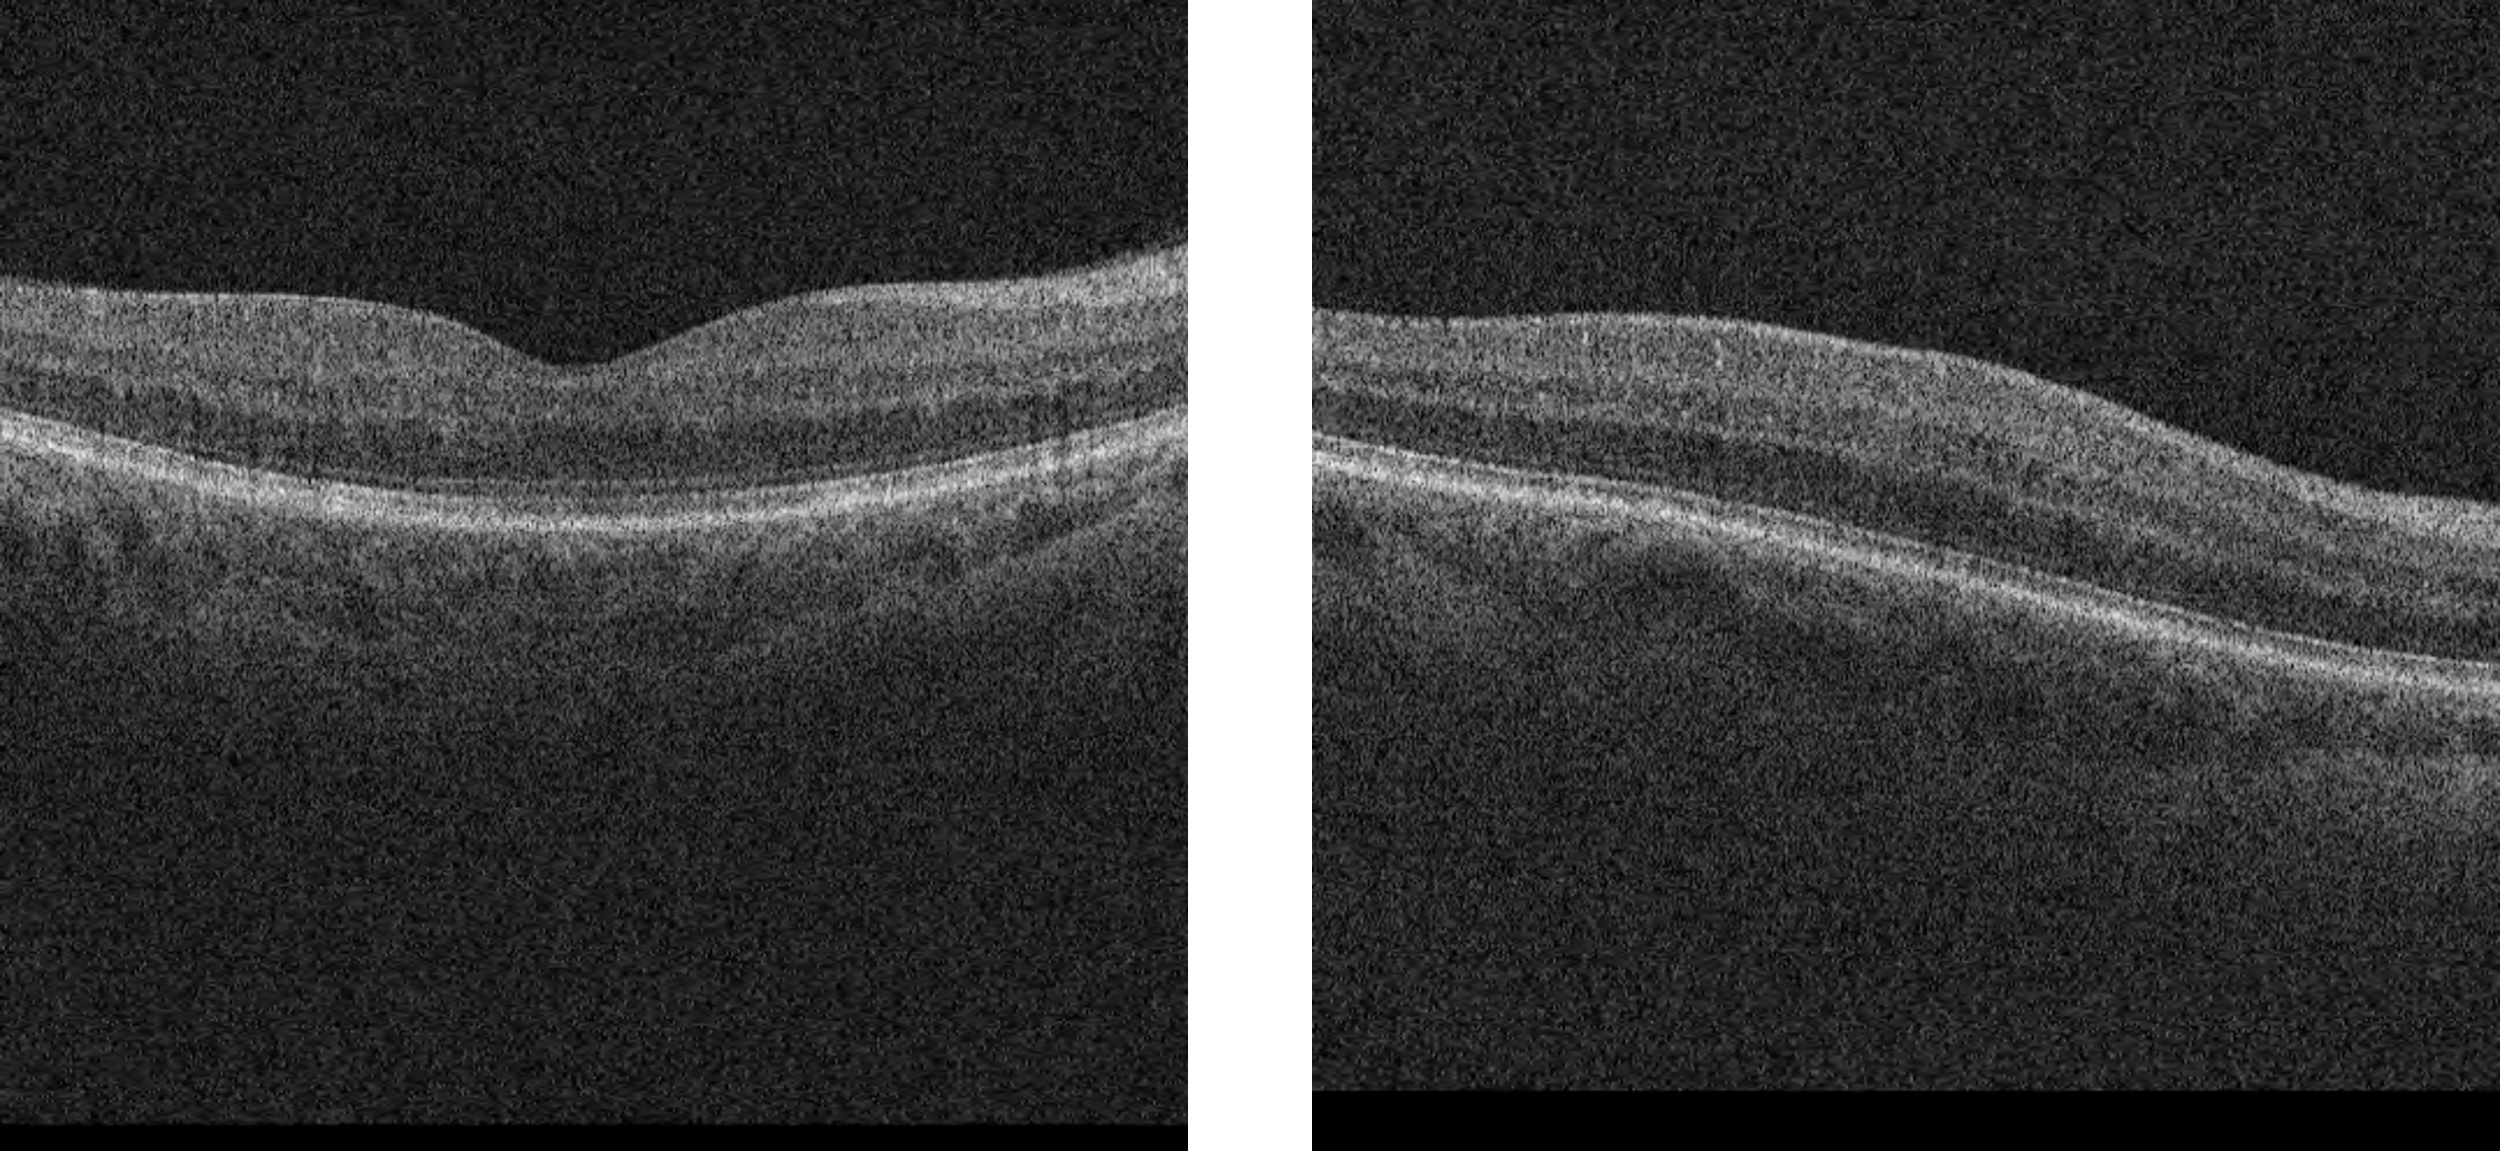
\includegraphics[width=0.7\linewidth]{figures/DifferentRetinaOrientation.png}
	\caption{Example of two B-scans in which the retina is oriented differently. The retina present in the right image is significantly more inclined. Both B-scans were obtained using a Cirrus device and do not present fluid.}
	\label{fig:DifferentRetinaOrientation}
\end{figure}

\begin{figure}[!ht]
	\centering
	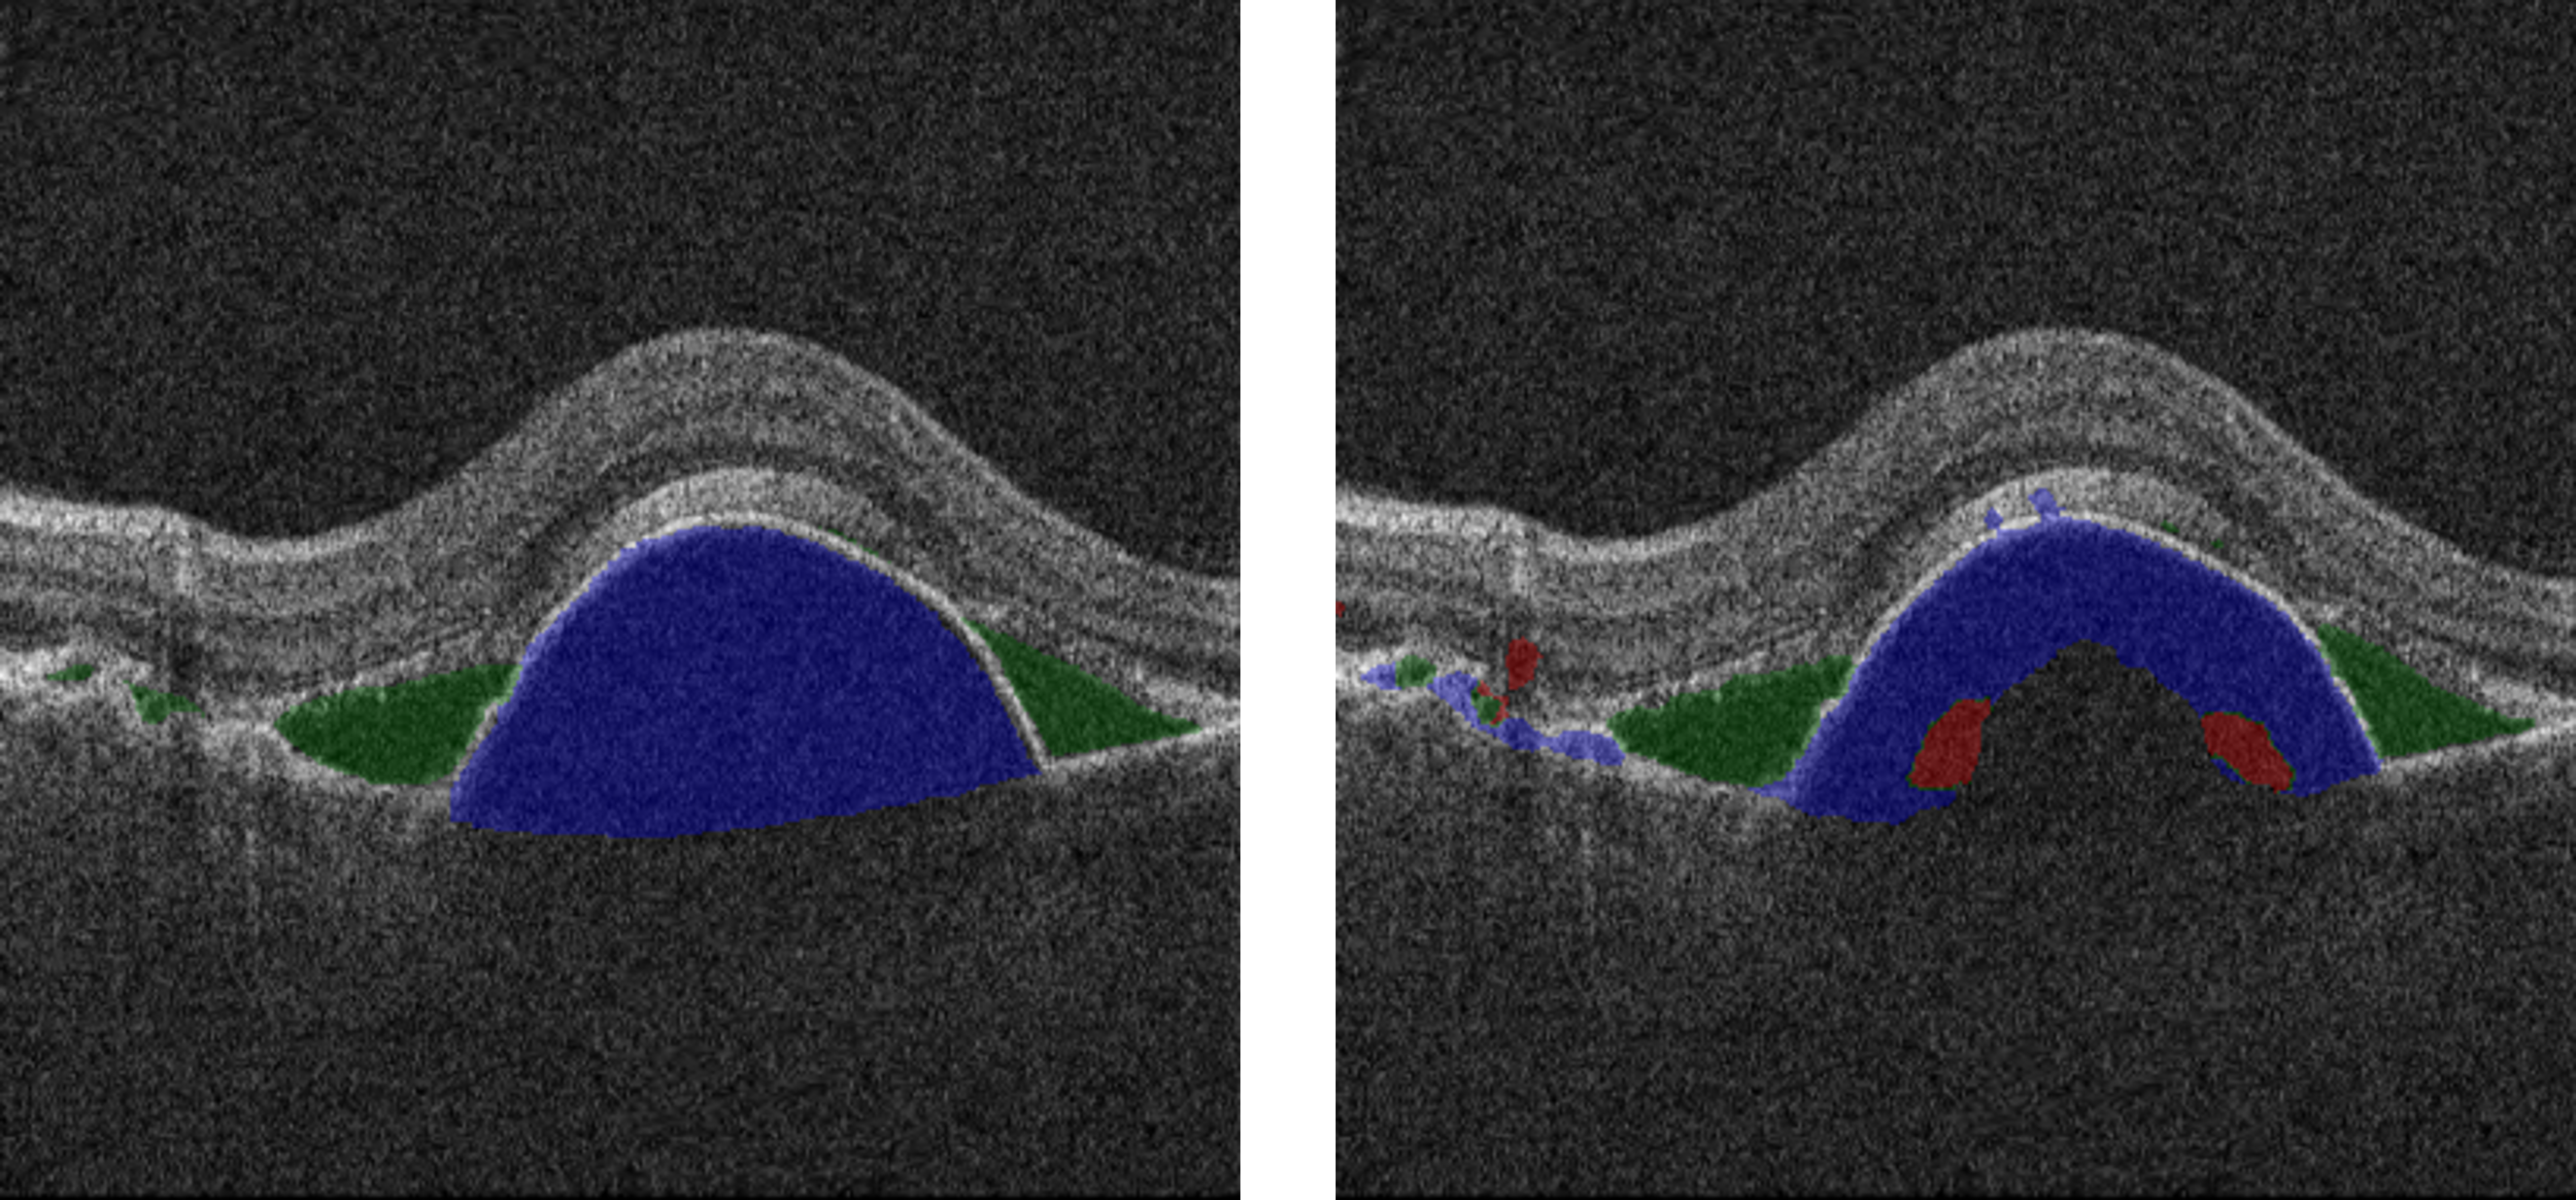
\includegraphics[width=0.7\linewidth]{figures/SegmentationErrorsNoRotation.png}
	\caption{Segmentation errors in Cirrus B-scans when trained without random rotations, in the same B-scan as in Figure \ref{fig:CirrusSegmentationErrors}. In the left, the GT masks are shown, while in the right the predicted masks are exhibited.}
	\label{fig:SegmentationErrorsNoRotation}
\end{figure}

In order to find an equilibrium between the robustness that training a model with rotated patches brings and the respect for the vertical order and relationships of the fluids, new runs were performed with a maximum $5^{\circ}$ rotation combined with the horizontal flipping. This rotation does not remove as much information from the patches as a $10^{\circ}$ rotation. The results obtained in these runs are shown in Table \ref{tab:Experiment1.3SevenPatches5DegreeRotation}.

\begin{table*}[!ht]
	\caption{Dice scores for every vendor and fluid using seven vertical patches. In these runs, horizontal flipping and $5^{\circ}$ rotation were used, instead of the usual $10^{\circ}$. The results obtained in Runs 21 and 22 are also shown, enabling a smoother comparison.}
	\centering
	\resizebox{\textwidth}{!}{\begin{tabular}{|c|c|ccc|ccc|ccc|c|c|c|c|}
		\hline
		% Headers
		\multirow{2}{*}{\textbf{Runs}} & 
		\multirow{2}{*}{\textbf{VF}} & 
		\multicolumn{3}{c|}{\textbf{Cirrus}} & 
		\multicolumn{3}{c|}{\textbf{Spectralis}} & 
		\multicolumn{3}{c|}{\textbf{Topcon}} & 
		\multicolumn{1}{c|}{\multirow{2}{*}{\textbf{IRF}}} & 
		\multirow{2}{*}{\textbf{SRF}} & 
		\multirow{2}{*}{\textbf{PED}} & 
		\multirow{2}{*}{\textbf{Fluid}} \\ \cline{3-11} & &
		\multicolumn{1}{c}{\textbf{IRF}} & 
		\multicolumn{1}{c}{\textbf{SRF}} & 
		\textbf{\textbf{PED}} & 
		\multicolumn{1}{c}{\textbf{IRF}} & 
		\multicolumn{1}{c}{\textbf{SRF}} & 
		\textbf{PED} & 
		\textbf{IRF} & 
		\textbf{SRF} & 
		\textbf{PED} & 
		\multicolumn{1}{c|}{} & & & \\ 
		
		\hline
		
		\textbf{Run 29} & 2 & \multicolumn{1}{c|}{0.497} & \multicolumn{1}{c|}{0.783} & 0.609 & \multicolumn{1}{c|}{0.763} & \multicolumn{1}{c|}{0.851} & 0.822 & \multicolumn{1}{c|}{0.832} & \multicolumn{1}{c|}{\textbf{0.904}} & 0.799 & 0.658 & 0.836 & 0.712 & 0.666 \\
		
		\textbf{Run 30} & 3 & \multicolumn{1}{c|}{0.475} & \multicolumn{1}{c|}{0.747} & 0.613 & \multicolumn{1}{c|}{0.656} & \multicolumn{1}{c|}{0.846} & 0.757 & \multicolumn{1}{c|}{\textbf{0.856}} & \multicolumn{1}{c|}{0.869} & \textbf{0.835} & 0.646 & 0.809 & 0.720 & 0.646 \\
		
		\textbf{Run 31} & 4 & \multicolumn{1}{c|}{0.643} & \multicolumn{1}{c|}{0.709} & 0.747 & \multicolumn{1}{c|}{0.627} & \multicolumn{1}{c|}{0.800} & 0.635 & \multicolumn{1}{c|}{0.457} & \multicolumn{1}{c|}{0.599} & 0.529 & 0.560 & 0.673 & 0.638 & 0.523 \\
		
		\textbf{Run 32} & 0 & \multicolumn{1}{c|}{\textbf{0.794}} & \multicolumn{1}{c|}{\textbf{0.878}} & \textbf{0.770} & \multicolumn{1}{c|}{\textbf{0.807}} & \multicolumn{1}{c|}{\textbf{0.902}} & \textbf{0.862} & \multicolumn{1}{c|}{0.796} & \multicolumn{1}{c|}{0.842} & 0.830 & \textbf{0.797} & \textbf{0.869} & \textbf{0.808} & \textbf{0.698} \\
		
		\hline
		
		\textbf{Set 7} & - & \multicolumn{1}{c|}{0.60} & \multicolumn{1}{c|}{0.78} & 0.68 & \multicolumn{1}{c|}{0.71} & \multicolumn{1}{c|}{0.85} & 0.77 & \multicolumn{1}{c|}{0.74} & \multicolumn{1}{c|}{0.80} & 0.75 & 0.67 & 0.80 & 0.72 & 0.63 \\
		
		\hline
		\hline
		
		\textbf{Run 21} & 2 & \multicolumn{1}{c|}{0.556} & \multicolumn{1}{c|}{0.837} & 0.672 & \multicolumn{1}{c|}{0.761} & \multicolumn{1}{c|}{0.853} & 0.848 & \multicolumn{1}{c|}{0.829} & \multicolumn{1}{c|}{0.908} & 0.858 & 0.685 & 0.864 & 0.767 & 0.681 \\

		\textbf{Run 22} & 3 & \multicolumn{1}{c|}{0.734} & \multicolumn{1}{c|}{0.855} & 0.836 & \multicolumn{1}{c|}{0.636} & \multicolumn{1}{c|}{0.846} & 0.689 & \multicolumn{1}{c|}{0.686} & \multicolumn{1}{c|}{0.781} & 0.731 & 0.700 & 0.822 & 0.771 & 0.672 \\

		\hline
			
	\end{tabular}}
	\label{tab:Experiment1.3SevenPatches5DegreeRotation}
\end{table*}

When looking at the results in Table \ref{tab:Experiment1.3SevenPatches5DegreeRotation}, the runs trained using a maximum $10^{\circ}$ rotation attain a better Dice coefficient than those that are trained using $5^{\circ}$. However, it is important to also compare the performances only in the slices that have fluid, which are shown in Table \ref{tab:Experiment1.3SevenPatches5DegreeRotationFluid}.

\begin{table*}[!ht]
	\caption{Dice scores for every vendor and fluid using seven vertical patches. The mean scores are calculated only for the B-scans that contain that fluid. For example, Cirrus IRF is the mean of the IRF Dice coefficient across all the Cirrus slices in the validation fold that contain IRF. The transformations utilized were the same as in Table \ref{tab:Experiment1.3SevenPatches5DegreeRotation}.}
	\centering
	\resizebox{\textwidth}{!}{\begin{tabular}{|c|c|ccc|ccc|ccc|c|c|c|c|}
			\hline
			% Headers
			\multirow{2}{*}{\textbf{Runs}} & 
			\multirow{2}{*}{\textbf{VF}} & 
			\multicolumn{3}{c|}{\textbf{Cirrus}} & 
			\multicolumn{3}{c|}{\textbf{Spectralis}} & 
			\multicolumn{3}{c|}{\textbf{Topcon}} & 
			\multicolumn{1}{c|}{\multirow{2}{*}{\textbf{IRF}}} & 
			\multirow{2}{*}{\textbf{SRF}} & 
			\multirow{2}{*}{\textbf{PED}} & 
			\multirow{2}{*}{\textbf{Fluid}} \\ \cline{3-11} & &
			\multicolumn{1}{c}{\textbf{IRF}} & 
			\multicolumn{1}{c}{\textbf{SRF}} & 
			\textbf{\textbf{PED}} & 
			\multicolumn{1}{c}{\textbf{IRF}} & 
			\multicolumn{1}{c}{\textbf{SRF}} & 
			\textbf{PED} & 
			\textbf{IRF} & 
			\textbf{SRF} & 
			\textbf{PED} & 
			\multicolumn{1}{c|}{} & & & \\ 
			
			\hline
			
			\textbf{Run 29} & 2 & \multicolumn{1}{c|}{0.499} & \multicolumn{1}{c|}{0.730} & \textbf{0.603} & \multicolumn{1}{c|}{0.596} & \multicolumn{1}{c|}{0.854} & 0.583 & \multicolumn{1}{c|}{\textbf{0.696}} & \multicolumn{1}{c|}{0.629} & 0.577 & 0.575 & 0.731 & 0.588 & 0.645 \\

			
			\textbf{Run 30} & 3 & \multicolumn{1}{c|}{0.535} & \multicolumn{1}{c|}{0.675} & 0.584 & \multicolumn{1}{c|}{0.519} & \multicolumn{1}{c|}{0.837} & 0.592 & \multicolumn{1}{c|}{0.646} & \multicolumn{1}{c|}{\textbf{0.735}} & 0.605 & 0.561 & 0.721 & 0.595 & 0.623 \\
			

			\textbf{Run 31} & 4 & \multicolumn{1}{c|}{\textbf{0.691}} & \multicolumn{1}{c|}{0.637} & 0.602 & \multicolumn{1}{c|}{0.619} & \multicolumn{1}{c|}{\textbf{0.899}} & 0.623 & \multicolumn{1}{c|}{0.506} & \multicolumn{1}{c|}{0.651} & \textbf{0.656} & 0.603 & 0.709 & \textbf{0.635} & \textbf{0.646} \\
			
			
			\textbf{Run 32} & 0 & \multicolumn{1}{c|}{0.627} & \multicolumn{1}{c|}{\textbf{0.815}} & 0.590 & \multicolumn{1}{c|}{\textbf{0.705}} & \multicolumn{1}{c|}{0.808} & \textbf{0.646} & \multicolumn{1}{c|}{0.563} & \multicolumn{1}{c|}{0.489} & 0.521 & \textbf{0.627} & \textbf{0.761} & 0.585 & 0.645 \\

			
			\hline
			
			\textbf{Set 7} & - & \multicolumn{1}{c|}{0.61} & \multicolumn{1}{c|}{0.74} & 0.59 & \multicolumn{1}{c|}{0.65} & \multicolumn{1}{c|}{0.85} & 0.65 & \multicolumn{1}{c|}{0.58} & \multicolumn{1}{c|}{0.62} & 0.55 & 0.60 & 0.75 & 0.59 & 0.64 \\

			\hline
			\hline
			
			\textbf{Run 21} & 2 & \multicolumn{1}{c|}{0.626} & \multicolumn{1}{c|}{0.795} & 0.449 & \multicolumn{1}{c|}{0.681} & \multicolumn{1}{c|}{0.842} & 0.771 & \multicolumn{1}{c|}{0.613} & \multicolumn{1}{c|}{0.697} & 0.524 & 0.636 & 0.791 & 0.518 & 0.636 \\
			
			
			\textbf{Run 22} & 3 & \multicolumn{1}{c|}{0.720} & \multicolumn{1}{c|}{0.687} & 0.554 & \multicolumn{1}{c|}{0.653} & \multicolumn{1}{c|}{0.914} & 0.543 & \multicolumn{1}{c|}{0.569} & \multicolumn{1}{c|}{0.679} & 0.615 & 0.647 & 0.738 & 0.583 & 0.651 \\
			
			
			\hline
			
	\end{tabular}}
	\label{tab:Experiment1.3SevenPatches5DegreeRotationFluid}
\end{table*}

The results shown in Table \ref{tab:Experiment1.3SevenPatches5DegreeRotationFluid} depict comparable results between the models trained with rotations of $5^{\circ}$ and $10^{\circ}$ degrees. While the results still slightly favor those trained with $10^{\circ}$ rotation, the difference between models is much smaller than it was in Table \ref{tab:Experiment1.3SevenPatches5DegreeRotation}. The differences observed indicate that the Dice coefficient measured in the models trained with $10^{\circ}$ rotation leverage on the high capability of detecting fluid. 
\par
This model is particularly good at detecting which slices have and do not have fluid. When the model does not detect fluid in a slice that does not have fluid, the Dice coefficient for that slice is 1. Meanwhile, in case the slices do not have fluid but the model still detects fluid in them, the B-scan's Dice coefficient for that fluid is 0.
\par
Due to the large quantity of slices that do not have fluid, which is larger than the slices that have fluid, a segmentation model can considerably improve its Dice performance by enhancing its capability of detecting fluid. Despite the model trained with $5^{\circ}$ performing worse at detecting fluid, most of these wrongful predictions are just a small quantity of sparse pixels (less than 100 pixels in each $496 \times 512$ image).
\par
It is also of interest to look into the predictions made by each model. While the Dice coefficient is a good metric to represent the models performance, some relevant segmentation characteristics can not be expressed by this measurement.
\par
When looking at the predictions made by both models, the model trained with $5^{\circ}$ rotations attains performances that are closer to the GT. An example of this can be seen in Figure \ref{fig:SegmentationsComparisonBetweenDifferentRotations}, where a comparison between the predictions made by different models are shown. In this image, it is seen that the masks predicted (middle image) by the model trained with $10^{\circ}$ rotation segments all the PED region, but also segments much more PED overall. Meanwhile, the model trained with $5^{\circ}$ rotation also identifies the PED region correctly, but segments less PED in the image (right image). The segmentation of IRF and SRF are really similar between both models.

\begin{figure}[!ht]
	\centering
	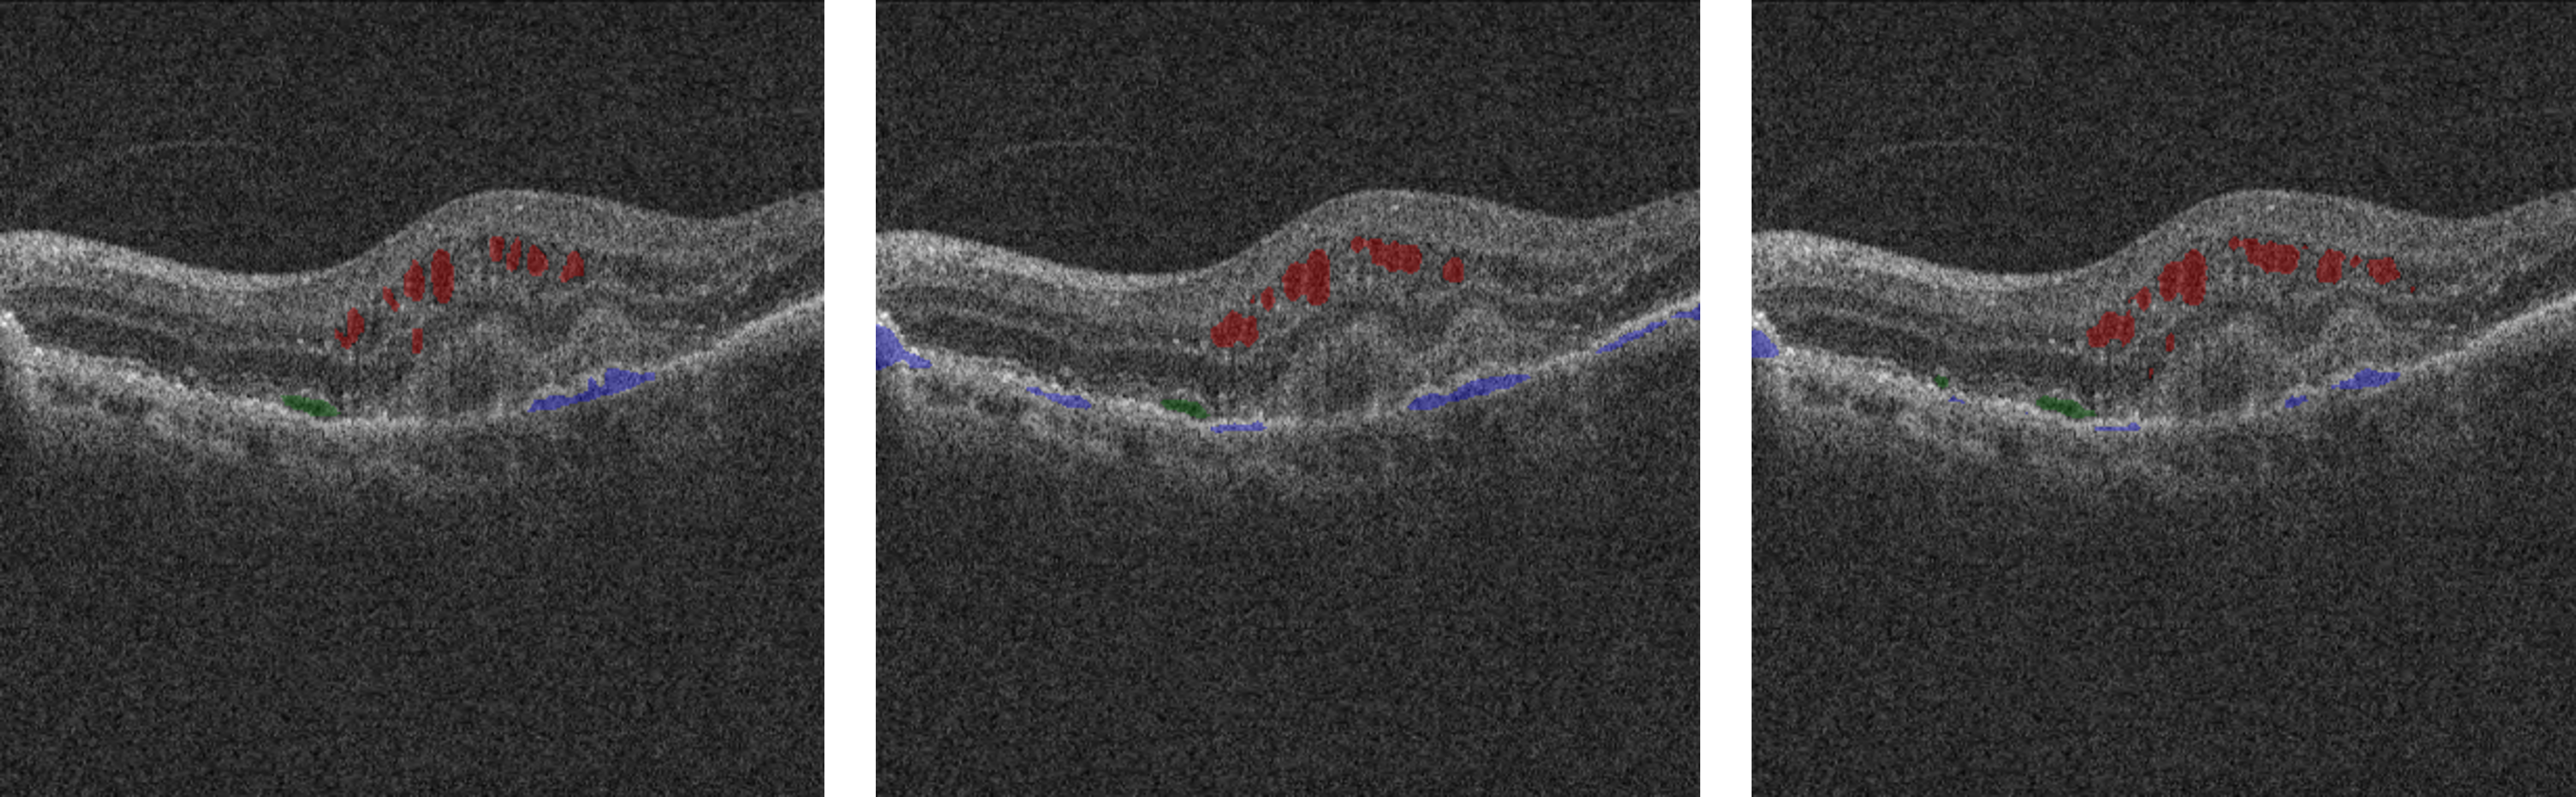
\includegraphics[width=1.0\linewidth]{figures/SegmentationsComparisonBetweenDifferentRotations.png}
	\caption{Predictions by the models trained using $5^{\circ}$ (middle image) and $10^{\circ}$ (right image) rotations, compared with the respective GT (left image).}
	\label{fig:SegmentationsComparisonBetweenDifferentRotations}
\end{figure}

This is an example of how the model trained with $5^{\circ}$ rotations tends to be more conservative in the fluid segmentation, despite not being as good at identifying fluid in the B-scans. For this reason, it was expected that this model would perform better on unseen data than the model trained with $10^{\circ}$ which tends to oversegment. Therefore, the maximum rotation selected for further experiments was $5^{\circ}$.
\par
Following the experiments that applied a $5^{\circ}$ rotation to the seven vertical patches extracted from each B-scan, additional runs made using the same rotation but with only four patches extracted from each B-scan instead. The objective of these runs was to verify if model still performs better on seven patches than on four patches when the applied rotation is changed from $10^{\circ}$ to $5^{\circ}$. The results are shown in Table \ref{tab:Experiment1.3FourPatches5DegreeRotation}.

\begin{table*}[!ht]
	\caption{Dice scores for every vendor and fluid using four vertical patches. The rotation applied in these runs was of $5^{\circ}$, instead of the previously used $10^{\circ}$. ``Set 7'' and the best performing run in this set (Run 32) are also shown, promoting an easier comparison between using four and seven patches. The underlined values correspond to the best performances between the models trained in Run 32 and Run 33.}
	\centering
	\resizebox{\textwidth}{!}{\begin{tabular}{|c|c|ccc|ccc|ccc|c|c|c|c|}
		\hline
		% Headers
		\multirow{2}{*}{\textbf{Runs}} & 
		\multirow{2}{*}{\textbf{VF}} & 
		\multicolumn{3}{c|}{\textbf{Cirrus}} & 
		\multicolumn{3}{c|}{\textbf{Spectralis}} & 
		\multicolumn{3}{c|}{\textbf{Topcon}} & 
		\multicolumn{1}{c|}{\multirow{2}{*}{\textbf{IRF}}} & 
		\multirow{2}{*}{\textbf{SRF}} & 
		\multirow{2}{*}{\textbf{PED}} & 
		\multirow{2}{*}{\textbf{Fluid}} \\ \cline{3-11} & &
		\multicolumn{1}{c}{\textbf{IRF}} & 
		\multicolumn{1}{c}{\textbf{SRF}} & 
		\textbf{\textbf{PED}} & 
		\multicolumn{1}{c}{\textbf{IRF}} & 
		\multicolumn{1}{c}{\textbf{SRF}} & 
		\textbf{PED} & 
		\textbf{IRF} & 
		\textbf{SRF} & 
		\textbf{PED} & 
		\multicolumn{1}{c|}{} & & & \\ 
			
		\hline
		
		\textbf{Run 33} & 2 & \multicolumn{1}{c|}{0.598} & \multicolumn{1}{c|}{\textbf{0.824}} & 0.719 & \multicolumn{1}{c|}{\textbf{0.805}} & \multicolumn{1}{c|}{0.873} & \underline{\textbf{0.887}} & \multicolumn{1}{c|}{\underline{\textbf{0.848}}} & \multicolumn{1}{c|}{\underline{\textbf{0.947}}} & \underline{\textbf{0.863}} & \textbf{0.720} & \underline{\textbf{0.874}} & \textbf{0.798} & \underline{\textbf{0.733}} \\
		
		\textbf{Run 34} & 3 & \multicolumn{1}{c|}{0.298} & \multicolumn{1}{c|}{0.701} & 0.436 & \multicolumn{1}{c|}{0.442} & \multicolumn{1}{c|}{0.785} & 0.720 & \multicolumn{1}{c|}{0.717} & \multicolumn{1}{c|}{0.814} & 0.746 & 0.477 & 0.757 & 0.599 & 0.530 \\
		
		\textbf{Run 35} & 4 & \multicolumn{1}{c|}{0.670} & \multicolumn{1}{c|}{0.796} & \textbf{0.850} & \multicolumn{1}{c|}{0.531} & \multicolumn{1}{c|}{0.825} & 0.701 & \multicolumn{1}{c|}{0.509} & \multicolumn{1}{c|}{0.703} & 0.674 & 0.582 & 0.759 & 0.754 & 0.578 \\
		
		\textbf{Run 36} & 0 & \multicolumn{1}{c|}{\textbf{0.695}} & \multicolumn{1}{c|}{0.816} & 0.737 & \multicolumn{1}{c|}{0.761} & \multicolumn{1}{c|}{\textbf{0.882}} & 0.838 & \multicolumn{1}{c|}{0.728} & \multicolumn{1}{c|}{0.867} & 0.775 & 0.719 & 0.846 & 0.769 & 0.635 \\
		
		\hline
		
		\textbf{Set 8} & - & \multicolumn{1}{c|}{0.57} & \multicolumn{1}{c|}{\textbf{0.78}} & \textbf{0.69} & \multicolumn{1}{c|}{0.63} & \multicolumn{1}{c|}{0.84} & \textbf{0.79} & \multicolumn{1}{c|}{0.70} & \multicolumn{1}{c|}{\textbf{0.83}} & \textbf{0.76} & 0.62 & \textbf{0.81} & \textbf{0.73} & 0.62 \\
		
		\hline
		\hline
		
		\textbf{Run 32} & 0 & \multicolumn{1}{c|}{\underline{0.794}} & \multicolumn{1}{c|}{\underline{0.878}} & \underline{0.770} & \multicolumn{1}{c|}{\underline{0.807}} & \multicolumn{1}{c|}{\underline{0.902}} & 0.862 & \multicolumn{1}{c|}{0.796} & \multicolumn{1}{c|}{0.842} & 0.830 & \underline{0.797} & 0.869 & \underline{0.808} & 0.698 \\
		
		\hline
		
		\textbf{Set 7} & - & \multicolumn{1}{c|}{\textbf{0.60}} & \multicolumn{1}{c|}{\textbf{0.78}} & 0.68 & \multicolumn{1}{c|}{\textbf{0.71}} & \multicolumn{1}{c|}{\textbf{0.85}} & 0.77 & \multicolumn{1}{c|}{\textbf{0.74}} & \multicolumn{1}{c|}{0.80} & 0.75 & \textbf{0.67} & 0.80 & 0.72 & \textbf{0.63} \\
		
		\hline
			
	\end{tabular}}
	\label{tab:Experiment1.3FourPatches5DegreeRotation}
\end{table*}

Contrasting with the results shown in Table \ref{tab:Experiment1.3FourPatches} and Table \ref{tab:Experiment1.3SevenVsThirteenPatches}, which show a significant improvement when using seven vertical patches over four, the results exhibited in Table \ref{tab:Experiment1.3FourPatches5DegreeRotation} present a similar performance between the models trained on four and seven vertical patches. The main performance differences are in the IRF segmentation, where the difference is more significant depending on the number of patches used, favoring the models trained with seven patches.
\par
However, it is necessary to select a single segmentation model to perform inference in the fold that was reserved. The best performing model from those trained with seven vertical patches obtained from each B-scan and a maximum rotation of $5^{\circ}$ is the model trained in Run 32. Meanwhile, the best performing model from ``Set 8'' is Run 33. In Table \ref{tab:Experiment1.3FourPatches5DegreeRotation}, the underlined values correspond to the best performance attained between Run 32 and 33.
\par
In most metrics, the model trained on Run 32 performs better than the model trained on Run 33. Nevertheless, both performances are really similar in most metrics, with the only significant difference being the IRF segmentation, which is superior in Run 32. It is important to note that the models were nor trained nor validated on the same data and an assumption that this would directly translate to the performance in unseen data was made. However, it is possible that the data in which one model was trained prepares it better for the data on the reserved fold. Therefore, the U-Net model selected to represent the multi-class segmentation approach was the one trained in Run 32. This model subsequently performed the inference in the unseen fold (fold 1) and its results are shown in Table \ref{tab:Experiment1.3FinalResults}. In this table, the rows correspond to the model performances on different sets of slices. In the first row the performance across all slices is considered. In the second row only the slices with the fluid indicated in the column are quantified, while in the third row only those that do not present that fluid are considered.

\begin{table*}[!ht]
	\caption{Dice scores for every vendor and fluid in the reserved fold (fold 1). The first row reports the mean Dice across all slices. The second row shows the mean for slices containing the fluid specified in the column, while the third shows the mean for the slices without that fluid.}
	\centering
	\resizebox{\textwidth}{!}{\begin{tabular}{|c|c|c|ccc|ccc|ccc|c|c|c|c|}
		\hline
		% Headers
		\multirow{2}{*}{\textbf{Runs}} &
		\multirow{2}{*}{\textbf{Slices}} &  
		\multirow{2}{*}{\textbf{VF}} & 
		\multicolumn{3}{c|}{\textbf{Cirrus}} & 
		\multicolumn{3}{c|}{\textbf{Spectralis}} & 
		\multicolumn{3}{c|}{\textbf{Topcon}} & 
		\multicolumn{1}{c|}{\multirow{2}{*}{\textbf{IRF}}} & 
		\multirow{2}{*}{\textbf{SRF}} & 
		\multirow{2}{*}{\textbf{PED}} & 
		\multirow{2}{*}{\textbf{Fluid}} \\ \cline{4-12} & & &
		\multicolumn{1}{c}{\textbf{IRF}} & 
		\multicolumn{1}{c}{\textbf{SRF}} & 
		\textbf{\textbf{PED}} & 
		\multicolumn{1}{c}{\textbf{IRF}} & 
		\multicolumn{1}{c}{\textbf{SRF}} & 
		\textbf{PED} & 
		\textbf{IRF} & 
		\textbf{SRF} & 
		\textbf{PED} & 
		\multicolumn{1}{c|}{} & & & \\ 
			
		\hline
			
		\multirow{3}{*}{\textbf{Run 32}} & All & 1 & \multicolumn{1}{c|}{0.852} & \multicolumn{1}{c|}{0.918} & 0.934 & \multicolumn{1}{c|}{0.645} & \multicolumn{1}{c|}{0.821} & 0.852 & \multicolumn{1}{c|}{0.818} & \multicolumn{1}{c|}{0.929} & 0.755 & 0.799 & 0.905 & 0.841 & 0.742 \\
		
		& Fluid & 1 & \multicolumn{1}{c|}{0.654} & \multicolumn{1}{c|}{0.799} & 0.767 & \multicolumn{1}{c|}{0.645} & \multicolumn{1}{c|}{0.687} & 0.703 & \multicolumn{1}{c|}{0.624} & \multicolumn{1}{c|}{0.744} & 0.588 & 0.641 & 0.756 & 0.716 & 0.702 \\
		
		& No Fluid & 1 & \multicolumn{1}{c|}{0.941} & \multicolumn{1}{c|}{0.972} & 0.978 & \multicolumn{1}{c|}{0.646} & \multicolumn{1}{c|}{0.889} & 0.885 & \multicolumn{1}{c|}{0.884} & \multicolumn{1}{c|}{0.960} & 0.766 & 0.873 & 0.952 & 0.862 & 0.786 \\
		
		\hline
			
	\end{tabular}}
	\label{tab:Experiment1.3FinalResults}
\end{table*}

The results shown in the table indicate that the model generalized well. The performance obtained in the reserved fold, whose data had not been used in training or validation, reveals the model's robustness across different fluids and vendors. Since the model performs equally well across the three vendors, a good cross-device generalization has been achieved. Therefore, the model is not dependent on the image quality of the B-scans to produce accurate predictions.
\par
The model behaved differently depending on the fluid expected to segment. The Dice coefficient was considerably larger in SRF and PED than in IRF. This is associated with the larger variety of IRF shape and position in the retina. IRF regions are usually irregular in shape, smaller, and less well-defined than the other fluids, often appearing as small structures. This fluid is also located between the retinal layers, making it harder for the model to distinguish from the surrounding tissue and often leading to labeling ambiguity. Still, the model attained a better performance in fluid segmentation than those seen in Table \ref{tab:Experiment1.3SevenPatches5DegreeRotationFluid}, where only fluid is considered.
\par
When considering all the slices, the Dice coefficient improves significantly, when compared to its performance where only slices with fluid are considered. At the same time, the Dice coefficient obtained in the slices without fluid is also better than the fluid segmentation. This reflects the greater difficulty of accurately segmenting the fluids, when compared to the task of detecting their presence. Since most slices in the dataset do not present fluid, an accurate detection of it can significantly increase the Dice mean across all slices, as explained previously.
\par
Overall, the performance obtained when validating in this unseen fold is significantly better than any other validation performance in previously seen in Table \ref{tab:Experiment1.3SevenPatches5DegreeRotation}. This indicates that the model did not overfit on training data, benefiting from the diversity introduced in training both through varying images and the transformations applied to them. This performance also benefits from selecting the best performing model in cross-validation, which allows the choice of a robust model. 
\par
In Figures \ref{fig:Experiment1FinalModelPredictionsCirrus}, \ref{fig:Experiment1FinalModelPredictionsSpectralis}, and \ref{fig:Experiment1FinalModelPredictionsTopcon}, some examples of predictions performed by the model in the unseen data are shown. In the IRF segmentations, it is seen that the model can not correctly identify the retinal tissue that separates the fluid regions and connects nearby fluid regions. The PED segmentation is marked by accurate delimitation of the large PED regions, with some predictions made in B-scans without PED. Lastly, SRF is the fluid in which the prediction segmentation more resembles the GT.
\par
The performance seen by this model in the reserved fold was subsequently compared with the best performing models from the following experiment.

\begin{figure}[!ht]
	\centering
	\includegraphics[width=0.9\linewidth]{figures/Experiment1FinalModelPredictionsCirrus.png}
	\caption{Predictions by the model trained on Run 32 in unseen Cirrus volumes of fold 1.}
	\label{fig:Experiment1FinalModelPredictionsCirrus}
\end{figure}

\begin{figure}[!ht]
	\centering
	\includegraphics[width=0.9\linewidth]{figures/Experiment1FinalModelPredictionsSpectralis.png}
	\caption{Predictions by the model trained on Run 32 in unseen Spectralis volumes of fold 1.}
	\label{fig:Experiment1FinalModelPredictionsSpectralis}
\end{figure}

\begin{figure}[!ht]
	\centering
	\includegraphics[width=0.9\linewidth]{figures/Experiment1FinalModelPredictionsTopcon.png}
	\caption{Predictions by the model trained on Run 32 in unseen Topcon volumes of fold 1.}
	\label{fig:Experiment1FinalModelPredictionsTopcon}
\end{figure}

\subsection{Experiment 2}
The results shown in this subsection correspond to the use of three separate U-Nets, one for each fluid, to perform multi-class fluid segmentation. In Experiment 2.1, the loss function was the same as in Experiment 1, while in Experiment 2.2 the loss function was changed to the weighted cross-entropy. The results in these experiments were compared with each other.

\subsubsection{Experiment 2.1}
In this experiment, for each fluid, eight models were trained. One model was trained for each fold in the multi-class 5-fold split and then one model was trained for each fold in a fluid-specific 5-fold split.
\par
Table \ref{tab:Experiment2IRF} illustrates the performance of the models trained to segment IRF, with the upper block corresponding to the models trained on the multi-class split while the second block shows the performances for the models trained on the split specifically made for IRF segmentation.

\begin{table*}[!ht]
	\caption{IRF Dice scores for every vendor. Runs 37 to 40 utilize the multi-class 5-fold split from Experiment 1, while the Runs 41 to 44 use the fluid-specific 5-fold split. The results are presented both for every slice and for the slices which contain IRF.}
	\centering
	\begin{tabular}{|c|c|cc|cc|cc|cc|}
			\hline
			\multirow{2}{*}{\textbf{Runs}} &
			\multirow{2}{*}{\textbf{VF}} & 
			\multicolumn{2}{c|}{\textbf{Cirrus}} & 
			\multicolumn{2}{c|}{\textbf{Spectralis}} & 
			\multicolumn{2}{c|}{\textbf{Topcon}} & 
			\multicolumn{2}{c|}{\textbf{IRF}} \\ 
			\cline{3-10} & &
			\multicolumn{1}{c}{\textbf{All}} &  
			\textbf{\textbf{Fluid}} & 
			\multicolumn{1}{c}{\textbf{All}} &  
			\textbf{\textbf{Fluid}} & 
			\multicolumn{1}{c}{\textbf{All}} & 
			\textbf{\textbf{Fluid}} & 
			\multicolumn{1}{c}{\textbf{All}} & 
			\textbf{\textbf{Fluid}}\\ 
			
			\hline
			
			\textbf{Run 37} & 2 & 0.478 & 0.634 & 0.695 & 0.669 & 0.735 & 0.569 & 0.604 & 0.625 \\
			
			\textbf{Run 38} & 3 & 0.536 & 0.452 & 0.514 & 0.588 & \textbf{0.820} & \textbf{0.706} & 0.637 & 0.553 \\
			
			\textbf{Run 39} & 4 & 0.545 & \textbf{0.683} & 0.617 & 0.670 & 0.540 & 0.484 & 0.552 & 0.600 \\
			
			\textbf{Run 40} & 0 & 0.576 & 0.619 & 0.695 & 0.682 & 0.661 & 0.599 & 0.628 & 0.628 \\
			
			\hline
			
			\textbf{Set 9} & - & 0.53 & 0.60 & 0.63 & 0.65 & 0.69 & \textbf{0.59} & 0.61 & 0.60 \\
			
			\hline
			\hline
			
			\textbf{Run 41} & 2 & \textbf{0.654} & 0.663 & 0.541 & 0.606 & 0.648 & 0.619 & 0.632 & 0.635 \\
			
			\textbf{Run 42} & 3 & 0.507 & 0.641 & \textbf{0.741} & 0.670 & 0.775 & 0.675 & \textbf{0.649} & \textbf{0.656} \\
			
			\textbf{Run 43} & 4 & 0.583 & 0.516 & 0.689 & 0.660 & 0.310 & 0.451 & 0.502 & 0.546 \\
			
			\textbf{Run 44} & 0 & 0.618 & 0.566 & 0.644 & \textbf{0.686} & 0.588 & 0.600 & 0.611 & 0.594 \\
			
			\hline
			
			\textbf{Set 10} & - & 0.59 & 0.60 & 0.65 & \textbf{0.66} & 0.58 & \textbf{0.59} & 0.60 & \textbf{0.61} \\
			
			\hline
			\hline
			
			\textbf{Set 7} & - & \textbf{0.60} & \textbf{0.61} & \textbf{0.71} & 0.65 & \textbf{0.74} & 0.58 & \textbf{0.67} & 0.60 \\
			
			\hline
			
	\end{tabular}
	\label{tab:Experiment2IRF}
\end{table*}

The results shown in this table follow a well defined trend: the IRF segmentation in the slices which contain this fluid performs similarly to the segmentation predicted by multi-class models, while the performance when considering all the slices is significantly worse.
\par
The Dice obtained in segmentation in the slices with IRF is really similar to the values obtained when training multi-class models, as the difference between the mean of the runs performed is around 0.01 for all vendors. Changing the split in which the models were trained barely made a difference in the performances' average. However, while the segmentation in slices with IRF almost did not change, the mean performance in all the slices saw a significant improvement in Cirrus and a slight increase in Spectralis, combined with a significant decrease in Topcon. 
\par
The reason Topcon behaves differently is because, overall, the volumes obtained with devices from this vendor present less fluid than the volumes obtained with the other devices. Therefore, the model has to analyze the Topcon images more carefully and be more attentive of the smaller details, as the fluid regions are not as big as those seen in the other vendors. This leads to the model being better at separating the slices with fluid from those that do not present fluid. As seen in Experiment 1, an effective detection of fluid can significantly improve the model's Dice coefficient. The implications this has in model performance's are also visible in the multi-class segmentation results, as shown in the performance differences in B-scans from Topcon between Table \ref{tab:Experiment1.3SevenPatches5DegreeRotation} and Table \ref{tab:Experiment1.3SevenPatches5DegreeRotationFluid}.
\par
When comparing the results across all slices between these binary models with the multi-class, it is seen a significant decrease in Dice coefficient in the models tasked to segment exclusively IRF. There are two main causes for this decrease, with the first being an increment in the number of voxels labeled as background. As the model attempts to exclusively segment IRF, all the voxels that are not labeled as IRF, are classified as background. This means that the regions of SRF and PED are also interpreted as background. The images in the dataset are predominantly composed of non-fluid voxels, but, by re-assigning the other fluids' voxels in the retina as background, the proportion of fluid voxels in the image, and particularly in the retina, becomes even smaller. As the number of background voxels increase, the more chances the model has of mislabeling them as fluid.
\par
The increased number of background voxels is further impacted with the lack of inter-class competition. This inter-class competition is particularly helpful in the segmentation of other ambiguous regions such as other fluids, which, in binary segmentation, is not contested by other classes. This does not incentive the model to learn the anatomical characteristics of the retina that are key to identifying the region corresponding to each fluid, often leading to over-segmentation. 
\par
This translates to a decrease in the IRF segmentation model's performance, particularly in the slices that do not present this fluid. The same performance decrease is also seen in SRF and PED, as shown further, due to the same reasons.
\par
Table \ref{tab:Experiment2SRF} shows the performance of the models trained on the same conditions as those trained to segment IRF, but now with the goal of segmenting SRF. Similarly, on the second block of this table, the models were trained using a 5-fold split specifically made to evenly distribute the OCT volumes according to the quantity of SRF in them.

\begin{table*}[!ht]
	\caption{SRF Dice scores for every vendor. Runs 45 to 48 utilize the multi-class 5-fold split from Experiment 1, while the Runs 49 to 52 use the fluid-specific 5-fold split. The results are presented both for every slice and for the slices which present SRF.}
	\centering
	\begin{tabular}{|c|c|cc|cc|cc|cc|}
		\hline
		\multirow{2}{*}{\textbf{Runs}} &
		\multirow{2}{*}{\textbf{VF}} & 
		\multicolumn{2}{c|}{\textbf{Cirrus}} & 
		\multicolumn{2}{c|}{\textbf{Spectralis}} & 
		\multicolumn{2}{c|}{\textbf{Topcon}} & 
		\multicolumn{2}{c|}{\textbf{SRF}} \\ 
		\cline{3-10} & &
		\multicolumn{1}{c}{\textbf{All}} &  
		\textbf{\textbf{Fluid}} & 
		\multicolumn{1}{c}{\textbf{All}} &  
		\textbf{\textbf{Fluid}} & 
		\multicolumn{1}{c}{\textbf{All}} & 
		\textbf{\textbf{Fluid}} & 
		\multicolumn{1}{c}{\textbf{All}} & 
		\textbf{\textbf{Fluid}}\\ 
		
		\hline
		
		\textbf{Run 45} & 2 & \textbf{0.866} & 0.784 & 0.882 & 0.826 & \textbf{0.956} & 0.645 & \textbf{0.899} & 0.774 \\
		
		\textbf{Run 46} & 3 & 0.599 & 0.574 & 0.741 & 0.843 & 0.820 & 0.737 & 0.705 & 0.666 \\
		
		\textbf{Run 47} & 4 & 0.769 & 0.645 & \textbf{0.874} & 0.873 & 0.845 & 0.689 & 0.816 & 0.728 \\
		
		\textbf{Run 48} & 0 & 0.667 & 0.795 & 0.765 & 0.776 & 0.773 & 0.643 & 0.723 & 0.765 \\
		
		\hline
		
		\textbf{Set 11} & - & 0.73 & 0.70 & 0.82 & 0.83 & \textbf{0.85} & 0.68 & 0.79 & 0.73 \\
		
		\hline		
		\hline
		
		\textbf{Run 49} & 2 & 0.509 & 0.758 & 0.617 & 0.793 & 0.759 & 0.607 & 0.613 & 0.745 \\
		
		\textbf{Run 50} & 3 & 0.743 & 0.733 & 0.776 & \textbf{0.885} & 0.901 & 0.801 & 0.807 & 0.779 \\
		
		\textbf{Run 51} & 4 & 0.720 & 0.722 & 0.864 & 0.875 & 0.816 & \textbf{0.803} & 0.781 & 0.809 \\
		
		\textbf{Run 52} & 0 & 0.775 & \textbf{0.872} & 0.810 & 0.826 & 0.879 & 0.676 & 0.819 & \textbf{0.826} \\
		
		\hline
		
		\textbf{Set 12} & - & 0.69 & \textbf{0.77} & 0.77 & 0.84 & 0.84 & \textbf{0.72} & 0.75 & \textbf{0.79} \\
		
		\hline
		\hline
		
		\textbf{Set 7} & - & \textbf{0.78} & 0.74 & \textbf{0.85} & \textbf{0.85} & 0.80 & 0.62 & \textbf{0.80} & 0.75 \\
		
		\hline
		
	\end{tabular}
	\label{tab:Experiment2SRF}
\end{table*}

As seen in this table, the performances in the segmentation of SRF in slices that contain this fluid have attained improved results when compared to those obtained using the multi-class model, especially when using the volume's distribution specific for SRF. In these conditions, the binary model significantly outperformed the multi-class model in the segmentation of slices with SRF from Cirrus and Topcon, while performing almost equally in the Spectralis slices.
\par
When looking at the models trained on the SRF 5-fold split, similarly to what happened in the IRF model, a significant performance decrease is seen when all the slices are considered. In these metrics, the model is outperformed by the multi-class model in every column except in the Topcon slices, where the performance increases. Similar to what was seen in the IRF segmentation, the performances in the Topcon volumes are not affected as much when performing binary segmentation due to the low quantity of fluid present in the OCT scans from this vendor.
\par
The results obtained using the multi-class split follow the same trend in Topcon. However, in Cirrus, it is seen a small increase in the Dice coefficient when considering all the slices. This is caused by the not so even volumes distribution, resulting in some folds having easier volumes for fluid detection, which have less fluid. This reflects in the high variance seen in the performance considering all slices in Cirrus. Contrasting, when the data is split equally, the dispersion is less pronounced, with only one outlier in that device (Run 49). Despite being more noticeable in Cirrus, Spectralis presents the same issue, where the results when using the multi-class split differ from what is expected and have sparser values.
\par
Overall, the Dice coefficient obtained in the SRF binary segmentation is better than the Dice obtained in the IRF. This same trend is also seen in Experiment 1, where SRF is the best performing fluid.
\par
The runs in which a binary segmentation U-Net was trained to segment PED are shown in Table \ref{tab:Experiment2PED}, where the behavior is comparable with the ones seen in IRF and SRF.

\begin{table*}[!ht]
	\caption{PED Dice scores for every vendor. Runs 53 to 56 utilize the multi-class 5-fold split from Experiment 1, while the Runs 57 to 60 use the fluid-specific 5-fold split. The results are presented both for every slice and for the slices which present PED.}
	\centering
	\begin{tabular}{|c|c|cc|cc|cc|cc|}
		\hline
		\multirow{2}{*}{\textbf{Runs}} &
		\multirow{2}{*}{\textbf{VF}} & 
		\multicolumn{2}{c|}{\textbf{Cirrus}} & 
		\multicolumn{2}{c|}{\textbf{Spectralis}} & 
		\multicolumn{2}{c|}{\textbf{Topcon}} & 
		\multicolumn{2}{c|}{\textbf{PED}} \\ 
		\cline{3-10} & &
		\multicolumn{1}{c}{\textbf{All}} &  
		\textbf{\textbf{Fluid}} & 
		\multicolumn{1}{c}{\textbf{All}} &  
		\textbf{\textbf{Fluid}} & 
		\multicolumn{1}{c}{\textbf{All}} & 
		\textbf{\textbf{Fluid}} & 
		\multicolumn{1}{c}{\textbf{All}} & 
		\textbf{\textbf{Fluid}}\\ 
		
		\hline
		
		\textbf{Run 53} & 2 & 0.305 & 0.482 & 0.555 & 0.623 & 0.626 & 0.552 & 0.459 & 0.522 \\
		
		\textbf{Run 54} & 3 & 0.447 & 0.508 & 0.437 & 0.628 & \textbf{0.769} & 0.623 & 0.563 & 0.583 \\
		
		\textbf{Run 55} & 4 & 0.368 & 0.594 & 0.346 & 0.566 & 0.328 & 0.618 & 0.348 & 0.600 \\
		
		\textbf{Run 56} & 0 & 0.484 & 0.547 & 0.326 & 0.639 & 0.697 & 0.460 & 0.534 & 0.545 \\
		
		\hline
		
		\textbf{Set 13} & - & 0.40 & 0.53 & 0.42 & 0.61 & 0.61 & 0.56 & 0.48 & 0.56 \\
		
		\hline
		\hline
		
		\textbf{Run 57} & 2 & 0.357 & 0.561 & 0.304 & 0.720 & 0.456 & 0.593 & 0.381 & 0.594 \\
		
		\textbf{Run 58} & 3 & 0.232 & 0.581 & 0.305 & 0.574 & 0.361 & 0.568 & 0.292 & 0.574 \\
		
		\textbf{Run 59} & 4 & 0.456 & \textbf{0.648} & 0.345 & 0.601 & 0.588 & \textbf{0.775} & 0.499 & \textbf{0.703} \\
		
		\textbf{Run 60} & 0 & \textbf{0.515} & 0.620 & \textbf{0.558} & \textbf{0.769} & 0.672 & 0.529 & \textbf{0.580} & 0.630 \\
		
		\hline
		
		\textbf{Set 14} & - & 0.39 & \textbf{0.60} & 0.38 & \textbf{0.67} & 0.52 & \textbf{0.62} & 0.44 & \textbf{0.63} \\
		
		\hline
		\hline
		
		\textbf{Set 7} & - & \textbf{0.68} & 0.59 & \textbf{0.77} & 0.65 & \textbf{0.75} & 0.55 & \textbf{0.72} & 0.59 \\
		
		\hline
		
	\end{tabular}
	\label{tab:Experiment2PED}
\end{table*}

In the binary segmentation of PED, the Dice coefficients obtained in the segmentation of slices with this fluid attained slightly better results when compared with those obtained in Experiment 1. However, this is only true when using the 5-fold split specifically made for this fluid. As seen in the previous experiments, the performance declines when considering all the slices.
\par
In the context of PED, it is important to understand the distribution of the fluid across the OCT volumes. While in IRF and SRF all volumes contain at least one of these fluids, in varying quantities, PED appears only in a smaller number of volumes and, in general, in large quantities. This makes the fair division across folds harder, since in each fold the B-scans that compose it are either with a large deformation caused by PED or, in most cases, without PED at all. This happens because most of the OCT volumes that present PED are in severe cases, where large quantities of all fluids appear. This large intra-class variability significantly affects the performance as it increases the difficulty of segmentation, leading to multiple occurrences of oversegmentation.
\par
This uneven distribution contributes to a poor performance when using all slices. It was already exposed that the models attained better fluid detection when dealing with smaller quantities of fluid, which resulted in a better detection performance in Topcon, where IRF and SRF appear in smaller areas. Now, when dealing with PED, the same trend is seen. However, in the other vendors, where PED appears in a larger quantity, the regions with this fluid generally occupy either larger areas or do not appear at all. This confuses the models, often leading to a segmentation of PED in slices where it is not present. This issue did not affect multi-class segmentation as the model capability of understanding the retina anatomy was more developed, as it was required to attribute the correct label to each voxel, which motivated the association between PED regions and the deformations seen in the retina.
\par
This translates to a good performance in the slices with fluid, but poor performance when all slices are considered. When the data partition is made specifically for PED, the quantity of fluid is fair in training and validation and the performances tend to what is expected: a significant decrease when all slices are considered, when compared to the segmentation in the slices with fluid, where the performance is decent. When using the multi-class segmentation split, fluid is not as evenly distributed, resulting in folds with more slices with PED and other folds with more slices without this fluid. In this case, and particularly in Topcon, models trained in folds that contain less fluid perform better at detecting fluid. For example, in Run 54, the models are trained on Topcon volumes with lower quantities of PED while fold 4 contains larger amounts, leading to correct detection of fluid in B-scans without any voxels labeled with this fluid. Inversely, in Run 55, the validation fold is composed of Topcon volumes with small amounts of PED, but trained on volumes with larger quantities. This results in oversegmentation in validation, thus attaining small Dice values when considering all the slices, but a decent score in the slices that have PED.
\par
In order to compare the results from this Experiment to the ones obtained in Experiment 1, three models had to be selected: one for IRF, one for SRF, and one for PED. Since the results obtained in Experiment 2.2 were much worse than the results reached in this experiment, the models selected for the inference in the unseen fold were selected from the runs performed in Experiment 2.1.
\par
From the models trained for IRF segmentation, ranging from Run 37 to Run 44, the model which obtained the best performance was the one trained on Run 42, as seen in Table \ref{tab:Experiment2IRF}. This model reached the best average performance in the segmentation of IRF both in all slices and when only slices with IRF were considered. In the other metrics, this model's performance were consistently similar to the best performing model in each metric. When compared to the average model from ``Set 7'', this model reached better performances in most metrics.
\par
The model selected to infer the SRF masks in the unseen fold was the model trained on Run 52. This model was the best performing SRF model in fluid segmentation in slices where SRF is present. In the other metrics, it performed closely to the best models, surpassing the average model from ``Set 7'' in most metrics.
\par
In PED, the selected model was the one trained on Run 59. This model was the best model in PED segmentation in slices that contain this fluid, with a significant difference from the other models. When considering all the slices, the model was the second best, but with a weak performance. Regarding the slices with fluid, this model outperformed the average from ``Set 7'' in all vendors. However, similar to all the other models trained for the binary segmentation of PED, it achieved a significantly worse performance when compared to the ones obtained in multi-class.
\par
When merging the masks from three independent binary segmentation models with the goal of outputting a multi-class segmentation, overlaps may occur, where multiple models assign different fluid labels to the same voxel. To resolve this conflict, two alternatives were explored in this fold: a priority-based approach, where the SRF takes precedence over IRF, which in turn takes precedence over PED; and a probability-based approach, where the predicted probabilities for the voxel are compared, attributing the label with highest predicted probability to it. 
\par
The results obtained using the three selected models are shown in Table \ref{tab:Experiment2FinalResults}, where the first block corresponds to the results when using the priority-based merging approach and the second block presents the results when using the probability-based approach.

\begin{table*}[!ht]
	\caption{Dice scores for every vendor and fluid in the reserved fold (fold 1), using the models from Runs 42, for IRF, 52, for SRF, and 59, for PED. The first block corresponds to the results when using the priority rule merging strategy, while the second block is associated with the results when using highest probability as the merging strategy. In each block, the first row reports the mean Dice across all slices. The second row shows the mean for slices containing the fluid specified in the column, while the third shows the mean for the slices without that fluid. The values marked in bold are the best values when corresponding rows are compared, so that, for example, the row ``All'' in the first block is compared to the row of same name in the second.}
	\centering
	\resizebox{\textwidth}{!}{\begin{tabular}{|c|c|c|ccc|ccc|ccc|c|c|c|c|}
			\hline
			% Headers
			\multirow{2}{*}{\textbf{Runs}} &
			\multirow{2}{*}{\textbf{Slices}} &  
			\multirow{2}{*}{\textbf{VF}} & 
			\multicolumn{3}{c|}{\textbf{Cirrus}} & 
			\multicolumn{3}{c|}{\textbf{Spectralis}} & 
			\multicolumn{3}{c|}{\textbf{Topcon}} & 
			\multicolumn{1}{c|}{\multirow{2}{*}{\textbf{IRF}}} & 
			\multirow{2}{*}{\textbf{SRF}} & 
			\multirow{2}{*}{\textbf{PED}} & 
			\multirow{2}{*}{\textbf{Fluid}} \\ \cline{4-12} & & &
			\multicolumn{1}{c}{\textbf{IRF}} & 
			\multicolumn{1}{c}{\textbf{SRF}} & 
			\textbf{\textbf{PED}} & 
			\multicolumn{1}{c}{\textbf{IRF}} & 
			\multicolumn{1}{c}{\textbf{SRF}} & 
			\textbf{PED} & 
			\textbf{IRF} & 
			\textbf{SRF} & 
			\textbf{PED} & 
			\multicolumn{1}{c|}{} & & & \\ 
			
			\hline
			
			\multirow{3}{*}{\parbox{2cm}{\textbf{Runs 42, 52, and 59}}} & All & 1 & \multicolumn{1}{c|}{0.693} & \multicolumn{1}{c|}{0.776} & 0.425 & \multicolumn{1}{c|}{0.587} & \multicolumn{1}{c|}{0.623} & 0.177 & \multicolumn{1}{c|}{0.808} & \multicolumn{1}{c|}{0.858} & \textbf{0.531} & 0.723 & 0.783 & 0.425 & \textbf{0.544} \\
			
			& Fluid & 1 & \multicolumn{1}{c|}{0.687} & \multicolumn{1}{c|}{\textbf{0.670}} & 0.573 & \multicolumn{1}{c|}{\textbf{0.660}} & \multicolumn{1}{c|}{\textbf{0.659}} & 0.632 & \multicolumn{1}{c|}{\textbf{0.634}} & \multicolumn{1}{c|}{\textbf{0.560}} & \textbf{0.484} & \textbf{0.661} & \textbf{0.640} & 0.570 & \textbf{0.639} \\
			
			& No Fluid & 1 & \multicolumn{1}{c|}{0.695} & \multicolumn{1}{c|}{0.824} & \textbf{0.387} & \multicolumn{1}{c|}{\textbf{0.520}} & \multicolumn{1}{c|}{0.605} & \textbf{0.075} & \multicolumn{1}{c|}{0.867} & \multicolumn{1}{c|}{0.907} & \textbf{0.534} & 0.752 & 0.830 & \textbf{0.402} & \textbf{0.440} \\
			
			\hline
			\hline
			
			\multirow{3}{*}{\parbox{2cm}{\textbf{Runs 42, 52, and 59}}} & All & 1 & \multicolumn{1}{c|}{\textbf{0.697}} & \multicolumn{1}{c|}{\textbf{0.787}} & \textbf{0.428} & \multicolumn{1}{c|}{\textbf{0.628}} & \multicolumn{1}{c|}{\textbf{0.631}} & \textbf{0.178} & \multicolumn{1}{c|}{\textbf{0.810}} & \multicolumn{1}{c|}{\textbf{0.864}} & \textbf{0.531} & \textbf{0.733} & \textbf{0.792} & \textbf{0.427} & \textbf{0.544} \\
			
			& Fluid & 1 & \multicolumn{1}{c|}{\textbf{0.688}} & \multicolumn{1}{c|}{0.663} & \textbf{0.586} & \multicolumn{1}{c|}{\textbf{0.660}} & \multicolumn{1}{c|}{0.646} & \textbf{0.636} & \multicolumn{1}{c|}{0.632} & \multicolumn{1}{c|}{0.537} & \textbf{0.484} & \textbf{0.661} & 0.627 & \textbf{0.578} & \textbf{0.639} \\
			
			& No Fluid & 1 & \multicolumn{1}{c|}{\textbf{0.701}} & \multicolumn{1}{c|}{\textbf{0.844}} & \textbf{0.387} & \multicolumn{1}{c|}{\textbf{0.520}} & \multicolumn{1}{c|}{\textbf{0.623}} & \textbf{0.075} & \multicolumn{1}{c|}{\textbf{0.870}} & \multicolumn{1}{c|}{\textbf{0.917}} & \textbf{0.534} & \textbf{0.766} & \textbf{0.844} & \textbf{0.402} & \textbf{0.440} \\
			
			\hline
			
	\end{tabular}}
	\label{tab:Experiment2FinalResults}
\end{table*}

The performances of the models shown in this table, indicate that the best merging strategy is the probability-based. In the slices that contain the evaluated fluid, the priority-based approach performs better in SRF, since it is the fluid of highest priority. Regarding IRF, in the slices where this fluid is present, the performance is equal for both approaches, while in PED the probability-based approach is better.
\par
However, when considering all the slices, the approach based on the probability of each model is significantly better. This is tied to the better performance in the slices that do not contain at least on type of fluid. In these slices, this approach prevents the segmentation of the fluids which are not present in the slice. These oversegmentations can be wrongfully predicted in the region of other fluids. However, since the models responsible for correctly segmenting this region are more confident than the models that are wrongfully segmenting it, the labels are attributed to the correct class.
\par
It is important to note that the ``Fluid'' column does not change when using different merging approaches. This is because the region of fluid segmented stays the same, since the only changes performed are in voxels contested by multiple fluids, and if all the fluids belonged to a single class, as considered in this column, no changes would be made.
\par
The overall segmentation performance was comparable to the values obtained in the validation folds, during training. In IRF, the model trained in Run 42 reaches better results in this unseen fold than in the fold in which it was originally validated. This is true when considering all the slices, just those with IRF, or the slices without IRF, which signals the good generalization by the model.
\par
In the segmentation of SRF, the model did not perform as good in this fold. The fluid detection was better, seen by the significant increase in Dice coefficient when considering all the slices instead of just those with fluid, which opposes the results obtained in the validation in Run 52, where the performance decreases in this situation. However, the segmentation worsened significantly in the slices with SRF, as the Dice coefficient dropped from 0.819 in its original validation fold to 0.627. Nevertheless, when considering all the slices, the Dice coefficients are still similar, largely due to the improved Dice in the slices without SRF.
\par
When segmenting IRF and SRF, the models benefited from a good generalization in fluid detection task, which surpassed the performances originally obtained in validation. However, in PED, where the models were the most sensitive in this matter, the performance in this task was worse. It is the only fluid in which the Dice is worse when considering all the slices than when considering just the slices with the fluid. This performance is tied to the model selected for PED segmentation. As seen in Table \ref{tab:Experiment2PED}, the model trained in Run 59 already presents a subpar performance in fluid detection, seen by the decrease in Dice coefficient when considering all the slices instead of those that contain PED. Therefore, the poor detection in unseen images is not unexpected. Note that the model selected detects fluid worse in the Spectralis volumes, similar to what was seen in the model validation. Similarly, the vendor in which the best performance is attained is the Topcon, where the model also performed best during validation. Moreover, all the PED models were expected to generalize worse in the unseen fold in the fluid detection task, due to the reasons previously presented that justify the lack of robustness in these models, such as the heterogeneous distribution of PED in OCT volumes.

\subsubsection{Experiment 2.2}

In this experiment, the loss function used in the training of the segmentation models was changed from a combination of a weighted cross-entropy and Dice coefficient of the foreground to the weighted cross-entropy. The results are shown in Table \ref{tab:Experiment2.2Results}, where only two runs were performed for the segmentation of IRF, one in each 5-fold split. 

\begin{table*}[!ht]
	\caption{IRF Dice scores for every vendor, using the binary segmentation U-Net for IRF. The loss function used in Runs 61 and 62 is the weighted cross-entropy. This model was trained on two different validation folds: validation fold 0 from the multi-class 5-fold split, and validation fold 4 from the 5-fold split specific for IRF. These results can be compared, respectively, to those obtained in Runs 40 and 43. The metrics are compared between rows with the same name, so that the values in bold are the best across the four experiments.}
	\centering
	\begin{tabular}{|c|c|c|c|c|c|c|}
			\hline
			% Headers
			\textbf{Runs} &
			\textbf{Slices} &  
			\textbf{VF} & 
			\textbf{Cirrus} & 
			\textbf{Spectralis} & 
			\textbf{Topcon} & 
			\textbf{IRF} \\ 
			
			\hline
			
			\multirow{3}{*}{\textbf{Run 61}} & All & 0 & 0.088 & 0.164 & 0.121 & 0.113 \\
			
			& Fluid & 0 & 0.320 & 0.390 & 0.472 & 0.378 \\
			
			& No Fluid & 0 & 0.002 & 0.044 & 0.041 & 0.024 \\
			
			\hline
			
			\multirow{3}{*}{\textbf{Run 62}} & All & 4 & 0.130 & 0.250 & 0.142 & 0.151 \\
			
			& Fluid & 4 & 0.399 & 0.531 & 0.549 & 0.466 \\
						
			& No Fluid & 4 & 0.000 & 0.052 & 0.053 & 0.030 \\
			
			\hline
			\hline
			
			\multirow{3}{*}{\textbf{Run 40}} & All & 0 & 0.576 & \textbf{0.695} & \textbf{0.661} & \textbf{0.628} \\
			
			& Fluid & 0 & \textbf{0.619} & \textbf{0.682} & \textbf{0.599} & \textbf{0.628} \\
			
			& No Fluid & 0 & 0.555 & 0.705 & \textbf{0.686} & \textbf{0.628} \\
			
			\hline
			
			\multirow{3}{*}{\textbf{Run 43}} & All & 4 & \textbf{0.583} & 0.689 & 0.310 & 0.502 \\
			
			& Fluid & 4 & 0.516 & 0.660 & 0.451 & 0.546 \\
			
			& No Fluid & 4 & \textbf{0.601} & \textbf{0.719} & 0.272 & 0.486 \\
			
			\hline
			
	\end{tabular}
	\label{tab:Experiment2.2Results}
\end{table*}

The results seen in the table are much worse than those obtained in the same conditions with the previous loss. In the slices with IRF, the segmentation was poor, but with a performance almost comparable to the values obtained in Run 40 and 43.
\par
However, what really worsens the overall performance is fluid detection. All the Dice coefficients in the slices with no fluid were inferior than 0.05, while most of the models studied in Experiment 2.1 reached values superior than 0.5.
\par
The reason these values were so low is related with the loss function used. By keeping the Dice loss as a component of the training loss, the model is highly penalized when predicting fluid in an image which does not have fluid. Whenever any fluid is predicted in such image, the Dice coefficient is 0. This motivates the model to carefully predict voxels in regions of the image where it highly believes there is fluid.
\par
When removing the Dice component from the loss, the wrongful predictions are only penalized by the cross-entropy component. This component does not penalize as much the predictions of fluid in empty images. The cross-entropy of each B-scan is calculated adjusted to the number of voxels belonging to a class in the image, as shown in \ref{Methods} Methods. Whenever a background voxel is wrongfully classified as fluid, the resulting penalty is really small, due to the large quantity of background voxels in the mask. Therefore, the incentive to not segment fluid in images which are solely composed of background is much smaller than it is when the Dice is considered. 
\par
The cross-entropy is much more useful when regularizing the wrong labeling, especially in fluid. Since this loss component is adjusted to the representation of each class in the image, wrongfully labeling a fluid region as another fluid or background brings a large penalty to the model. This is why it is combined with the Dice loss in the original loss: while the Dice ensures that the correct areas of fluid are segmented, the cross-entropy makes sure that the correct labels are assigned to each voxel. For this reason, most of the segmentation errors that are seen in the predictions made by the models trained in Run 61 and 62 are oversegmentations, and not as many incorrect labelings.

\subsubsection{Experiment 1 and Experiment 2 Comparison}

In order to compare Experiment 1 with Experiment 2, both their performances were presented in Table \ref{tab:Experiment1VsExperiment2}. These experiments are compared by evaluating each experiment's performance on the reserved fold. In the table, the first block corresponds to the performance obtained with the selected multi-class segmentation model, while the second block shows the performance of the combination of models from Experiment 2, with their masks combined in a probability-based approach.

\begin{table*}[!ht]
	\caption{Dice scores for every vendor and fluid in the reserved fold (fold 1), using the best models from Experiment 1 and Experiment 2. In Experiment 1, the model trained on Run 32 was selected, while in Experiment 2 the chosen models were those from Runs 42, for IRF, 52, for SRF, and 59, for PED. The rows with the same name must be compared with each other.}
	\centering
	\resizebox{\textwidth}{!}{\begin{tabular}{|c|c|c|ccc|ccc|ccc|c|c|c|c|}
			\hline
			% Headers
			\multirow{2}{*}{\textbf{Runs}} &
			\multirow{2}{*}{\textbf{Slices}} &  
			\multirow{2}{*}{\textbf{VF}} & 
			\multicolumn{3}{c|}{\textbf{Cirrus}} & 
			\multicolumn{3}{c|}{\textbf{Spectralis}} & 
			\multicolumn{3}{c|}{\textbf{Topcon}} & 
			\multicolumn{1}{c|}{\multirow{2}{*}{\textbf{IRF}}} & 
			\multirow{2}{*}{\textbf{SRF}} & 
			\multirow{2}{*}{\textbf{PED}} & 
			\multirow{2}{*}{\textbf{Fluid}} \\ \cline{4-12} & & &
			\multicolumn{1}{c}{\textbf{IRF}} & 
			\multicolumn{1}{c}{\textbf{SRF}} & 
			\textbf{\textbf{PED}} & 
			\multicolumn{1}{c}{\textbf{IRF}} & 
			\multicolumn{1}{c}{\textbf{SRF}} & 
			\textbf{PED} & 
			\textbf{IRF} & 
			\textbf{SRF} & 
			\textbf{PED} & 
			\multicolumn{1}{c|}{} & & & \\ 
			
			\hline

			\multirow{3}{*}{\textbf{Run 32}} & All & 1 & \multicolumn{1}{c|}{\textbf{0.852}} & \multicolumn{1}{c|}{\textbf{0.918}} & \textbf{0.934} & \multicolumn{1}{c|}{\textbf{0.645}} & \multicolumn{1}{c|}{\textbf{0.821}} & \textbf{0.852} & \multicolumn{1}{c|}{\textbf{0.818}} & \multicolumn{1}{c|}{\textbf{0.929}} & \textbf{0.755} & \textbf{0.799} & \textbf{0.905} & \textbf{0.841} & \textbf{0.742} \\
			
			& Fluid & 1 & \multicolumn{1}{c|}{0.654} & \multicolumn{1}{c|}{\textbf{0.799}} & \textbf{0.767} & \multicolumn{1}{c|}{0.645} & \multicolumn{1}{c|}{\textbf{0.687}} & \textbf{0.703} & \multicolumn{1}{c|}{0.624} & \multicolumn{1}{c|}{\textbf{0.744}} & \textbf{0.588} & 0.641 & \textbf{0.756} & \textbf{0.716} & \textbf{0.702} \\
			
			& No Fluid & 1 & \multicolumn{1}{c|}{\textbf{0.941}} & \multicolumn{1}{c|}{\textbf{0.972}} & \textbf{0.978} & \multicolumn{1}{c|}{\textbf{0.646}} & \multicolumn{1}{c|}{\textbf{0.889}} & \textbf{0.885} & \multicolumn{1}{c|}{\textbf{0.884}} & \multicolumn{1}{c|}{\textbf{0.960}} & \textbf{0.766} & \textbf{0.873} & \textbf{0.952} & \textbf{0.862} & \textbf{0.786} \\
			
			\hline
			\hline
			
			\multirow{3}{*}{\parbox{2cm}{\textbf{Runs 42, 52, and 59}}} & All & 1 & \multicolumn{1}{c|}{0.697} & \multicolumn{1}{c|}{0.787} & 0.428 & \multicolumn{1}{c|}{0.628} & \multicolumn{1}{c|}{0.631} & 0.178 & \multicolumn{1}{c|}{0.810} & \multicolumn{1}{c|}{0.864} & 0.531 & 0.733 & 0.792 & 0.427 & 0.544 \\
			
			& Fluid & 1 & \multicolumn{1}{c|}{\textbf{0.688}} & \multicolumn{1}{c|}{0.663} & 0.586 & \multicolumn{1}{c|}{\textbf{0.660}} & \multicolumn{1}{c|}{0.646} & 0.636 & \multicolumn{1}{c|}{\textbf{0.632}} & \multicolumn{1}{c|}{0.537} & 0.484 & \textbf{0.661} & 0.627 & 0.578 & 0.639 \\
			
			& No Fluid & 1 & \multicolumn{1}{c|}{0.701} & \multicolumn{1}{c|}{0.844} & 0.387 & \multicolumn{1}{c|}{0.520} & \multicolumn{1}{c|}{0.623} & 0.075 & \multicolumn{1}{c|}{0.870} & \multicolumn{1}{c|}{0.917} & 0.534 & 0.766 & 0.844 & 0.402 & 0.440 \\
			
			\hline
			
	\end{tabular}}
	\label{tab:Experiment1VsExperiment2}
\end{table*}

By looking at this table, the best segmentation performance becomes evident. The multi-class model consistently outperforms the binary models in across all fluids, vendors and slice groups.
\par
Regarding the performances in fluids, the multi-class segmentation performs better than the binary models in all fluids when all the slices are considered and when only the slices which do not contain a certain fluid are considered. The only metrics in which the binary models outperform the multi-class is the segmentation of IRF in slices which contain this fluid. In these metrics, the binary models attain small improvements over the multi-class model. This fluid was also the one with the best performance in the set of slices with IRF, in Experiment 2.1. However, the segmentation of IRF in the slices which contain this fluid is not enough to 
\par
The performances reached by the binary model in SRF are worse than those obtained with the multi-class, but still 

\par
It was seen in Experiment 2 

\section{Intermediate Slice Synthesis}\label{IntermediateSliceSynthesis}

\subsection{Experiment 3}

\subsection{Experiment 4}

\section{Fluid Volume Estimation}\label{FluidVolumeEstimation}

\subsection{Experiment 5}

\subsection{Experiment 6}